% Use the temporary template.
\documentclass[12pt]{aiaa-pretty}

\usepackage{amssymb,amsmath}
\usepackage{graphicx,float}
\usepackage{lettrine}
\usepackage{wasysym} % For double surface close integrals

\usepackage{setspace} 
\doublespacing
\usepackage{subfigure} %For side-by-side figures
\usepackage{epstopdf} %To read *.eps Files
\usepackage{multirow}

\usepackage[T1]{fontenc}
\usepackage[utf8]{inputenc}
%\usepackage{authblk}

% FOR TABLES
\usepackage{multirow}
\usepackage{array}
\newcolumntype{L}[1]{>{\raggedright\let\newline\\\arraybackslash\hspace{0pt}}m{#1}}
\newcolumntype{C}[1]{>{\centering\let\newline\\\arraybackslash\hspace{0pt}}m{#1}}
\newcolumntype{R}[1]{>{\raggedleft\let\newline\\\arraybackslash\hspace{0pt}}m{#1}}

\usepackage[linewidth=1pt]{mdframed}
\usepackage{lipsum}

% Author information
\author[Gobal and Grandhi]{ %
Koorosh Gobal\thanks{Graduate Research Assistant, Department of Mechanical and Materials Engineering, AIAA Student Member, gobal.2@wright.edu.} and
Ramana V. Grandhi\thanks{Distinguished Research Professor, Department of Mechanical and Materials Engineering, AIAA Fellow.}\\
\textit{Wright State University, Dayton, Ohio 45324}}

% Title
\title{High-Fidelity Aerodynamic Shape Optimization using Immersed Boundary Method}

% Abstract
\abstract{A continuous shape sensitivity formulation is developed for the aerodynamic design optimization on Cartesian structured mesh. The continuous sensitivity analysis enables the use of original solver for the solution of the sensitivity equations. The governing equations are the compressible laminar Navier-Stokes equations, and the effect of solid boundaries are modeled using an immersed boundary approach. The immersed boundary formulation decouples the mesh from the solid boundary definition; therefore, mesh update is not required throughout the shape optimization process. A detailed discussion of the implementation of continuous sensitivity analysis for the immersed boundary method is presented. This methodology is applied shape optimization of NACA 0012 airfoil at various flight condition. The sensitivity results are verified using the complex step method. The final paper will implement this methodology to compressible flows and will also include the verification of optimization results using NASA's FUN3D code.}


% Begin the document
\begin{document}
% Insert the title.
\maketitle
% ==========================================================================================
\section{Introduction}
Aerodynamic design optimization of aircraft heavily depends on the computational tools to rapidly and accurately evaluate different design configurations. This is critical in the transonic region since a small change in the wing shape leads to significant perturbation of aerodynamic properties of the wing. High-fidelity Computational Fluid Dynamic (CFD) tools have been a great interest in recent year due to improvement in computational power available to researchers. Faster computational cores reduce the simulation time of each CFD run which enables the use of CFD simulation in an optimization loop. Various optimization techniques can be applied to the aerodynamic design problem; however, the gradient-based optimization methods have proved themselves to be the most efficient approach. Gradient-based optimization requires calculating the sensitivity of the object function and constraints with respect to the design variables to update the design. The analytical sensitivity analysis can be done using a discrete or continuous approach.

Formulation of the analytical sensitivity methods requires derivation of sensitivity equations. These equations are obtained by differentiating the governing equations with respect to design variables such as the shape of the boundaries. Among the available methods, discrete analytical sensitivities is a popular approach, where the discretized system of governing equations are differentiated \cite{martins2013review}. It is necessary to modify the source-code of the black-box CFD/FEA solvers \cite{cross2014local}, this might not be possible due to lack of source codes availability. Continuum Sensitivity Analysis (CSA) on the other hand involves solving a set of partial differential equations named the continuum sensitivity equations (CSEs) to calculate analytical sensitivities. CSA has several computational efficiencies that other sensitivity formulations lack. Aurora and Haug \cite{Arora}, and later Dems and Mroz \cite{Dems-Mroz} were among the first to introduce CSA for structural problems. Liu and Canfield have employed CSA for shape optimization of nonlinear structures subject to an aeroelastic gust response \cite{liu2013equivalence}. They used the finite element method to solve the potential flow around an airfoil and applied CSA to find the airfoil pressure coefficient sensitivity with respect to the maximum camber.

In these works, body conforming grids were used to model the flow around the solid bodies. The conforming mesh methods consider the interface conditions as physical boundary conditions, which treat the interface location as part of the solution and requires meshes that conform to the interface. Owing to the movement and/or deformation of the solid structure, re-meshing (or mesh-updating) is needed as the solid boundaries move. The sensitivity analysis is also simplified when using a non-body conformal mesh since the mesh sensitivity is equal to zero. However, the shape boundary sensitivity is still required for this approach \cite{liu2013boundary}. The shortcoming of a body conforming grid generation and the additional cost of calculating mesh sensitivities motivate the current work to develop a method that does not require fluid domain mesh modification for the optimization iterations.

Most non-body conforming mesh techniques are based upon the framework of the Immersed Boundary (IB) methods where a numerically efficient Cartesian grid is used for the discretization of the fluid domain. The effect of solid boundaries can be handled in the continuous domain, i.e. before discretization, or by altering the linear system resulting from discretization in time and space, which is termed discrete forcing \cite{mittal2005immersed}. In the IB method, the boundary of an immersed solid is tracked by Lagrangian markers. Numerically, the communication between the solid and the fluid is obtained by spreading singular forces from the Lagrangian markers to nearby Cartesian grid nodes and interpolating the velocity from nearby Cartesian grid nodes to the Lagrangian markers with the use of discrete Dirac $\delta$ functions.

Most research that has been done on the IB method focused on the analysis aspects of the method, and the sensitivity analysis has not been extensively studied. Choi et al. calculated the surface pressure coefficients for high Reynolds number flow around an NACA 0012 airfoil \cite{choi2007immersed}. Fadlun et al. investigated the capability of this method to simulate high-Reynolds number turbulent flows in complex geometries. They chose an axisymmetric piston-cylinder assembly with a fixed central valve for this purpose \cite{fadlun2000combined}. Koehler et al. investigated the flow produced by rotation and translation of a cylinder using IB method in two dimensions \cite{koehler2015flows}. They were able to model various streaming jet regimes as a propulsive mechanism. Vanella et al. tested the accuracy of the IB method for the case of two falling plates \cite{vanella2010direct}. There has been limited research on the application of the IB method for optimization of the internal flows where the penalization technique was used to optimize the shape of the channels for fluid flow \cite{kreissl2012levelset} however, the developed methodology is only applicable to low Reynolds number flows and does not provide good accuracies near the solid boundaries.

In this research, we use continuum sensitivity analysis to calculate aerodynamic sensitivity to shape parameters, where the flow is modeled using the Navier-Stokes equations. The conventional immersed boundary methods often use a discrete Dirac function for transferring data between domains. This is not applicable when using continuum sensitivity analysis since the governing equations need to be continuously differentiable. Therefore, a continuous regularized delta function is developed to satisfy this need. The sensitivity analysis data is then used to the shape optimization of NACA 0012 and RAE 2822 airfoils in both compressible and incompressible flow. The solution using the IB method is compared with the FUN3D results which are based on body-conformal mesh generation and discrete sensitivity analysis.

% ==========================================================================================
\section{Numerical Approach}
% -.-.-.-.-.-.-.-.-.-.-.-.-.-.-.-.-.-.-.-.-.-.-.-.-.-.-.-.-.-.-.-.-.-.-.-.-.-.-.-.-.-.-.-.-
\subsection{Immersed Boundary Formulation}\label{subsec:IB}
Flow in a Cartesian domain, $\Omega$, containing an immersed boundary of Figure \eqref{fig:immersedBoundary}, is modeled by using the Navier-Stokes equations:
%
\begin{subequations}\label{eq:NS}
\begin{align}
	\rho^f \frac{\partial \mathbf{u}^f}{\partial t} + 
	\rho^f \mathbf{u}^f \cdot \nabla \mathbf{u}^f = 
	\nabla \cdot \mathbf{\sigma}^f +
	\rho^f \mathbf{f}^f
	\quad \quad &\text{: Conservation of momentum}
	\\
	\nabla \cdot \mathbf{u}^f = 0
	\quad \quad &\text{: Conservation of mass}
	\\
	\mathbf{\sigma}^f = 
	\mu \left[ \nabla \mathbf{u}^f + \left( \nabla \mathbf{u}^f \right)^T \right] - 
	p^f \mathbf{I}
	\quad \quad &\text{: Stress formula}
\end{align}
\end{subequations}
%
In the above equations, superscript \lq\emph{f}\rq\ corresponds to the fluid properties. In Equation \eqref{eq:NS} $\rho^f$, $\mathbf{u}^f$, $p^f$, and $\mathbf{f}^f$ correspond to the fluid density, velocity, pressure, and body forces, respectively. It should be noted that the immersed boundary forces are applied through the body force term $\mathbf{f}^f$. The forcing function, $\mathbf{f}^f$ is given by
%
\begin{equation}\label{eq:forceAtEulerian}
	\mathbf{f}^f(\mathbf{x}, t) = \int_\Omega \mathbf{f}^f (\mathbf{x}_k, t) \delta(\mathbf{x} - \mathbf{x}_k) d\mathbf{x}_k
\end{equation}
%
where $\delta(\mathbf{x} - \mathbf{x}_k)$ is a Dirac delta function; $\mathbf{x}_k$ are the locations of Lagrangian points placed over the immersed boundary; $\mathbf{f}^f(\mathbf{x}_k)$ is the Lagrangian force density; and $\mathbf{f}^f(\mathbf{x})$ is the Eulerian force that has non-zero values only over the immersed boundary.

The Lagrangian force terms are calculated using virtual boundary formulation proposed by Goldstein \cite{goldstein1993modeling}. The main idea of this method is to treat the embedded boundary by adding a force field to the fluid in such a way that the fluid takes the same velocity as the solid surface. Since the force field is not known a priori, it must be calculated in a feedback way as shown in Equation \eqref{eq:forcingFunction}. This model involves two imposed constants, $\alpha$ and $\beta$, which are chosen to be both negative and large enough in magnitude to force the fluid velocity to the interface velocity. The feedback forcing function $\mathbf{f}(\mathbf{x}_k, t)$ is given as
%
\begin{equation}\label{eq:forcingFunction}
	\mathbf{f}^f\left( \mathbf{x}_k, t \right) = 
	\alpha \int_0^t \left[ \mathbf{u}^f\left( \mathbf{x}_k, t \right) - \mathbf{U}\left( \mathbf{x}_k, t \right) \right]dt + 
	\beta \left[ \mathbf{u}^f\left( \mathbf{x}_k, t \right) - \mathbf{U}\left( \mathbf{x}_k, t \right) \right]
\end{equation}
%
where $\mathbf{u}^f\left( \mathbf{x}_k, t \right)$ is the velocity value from the Eulerian analysis calculated at the Lagrangian nodes. $\mathbf{U}\left( \mathbf{x}_k, t \right)$ is the velocity at the corresponding Lagrangian nodes, $\mathbf{x}_k$. For the case of a no-slip boundary condition ($\mathbf{U}\left( \mathbf{x}_k, t \right) = 0 $) the forcing function in Equation \eqref{eq:forcingFunction} tries to bring the velocity to zero on the boundary. $\mathbf{u}^f\left( \mathbf{x}_k, t \right)$ is calculated from its neighbouring Eulerian nodes by using the same delta function used in Equation \eqref{eq:forceAtEulerian}.
%
\begin{equation}\label{eq:velocityAtLagrangian}
	\mathbf{u}^f(\mathbf{x}_k, t) = \int_\Omega \mathbf{u}^f (\mathbf{x}, t) \delta(\mathbf{x} - \mathbf{x}_k) d\mathbf{x}
\end{equation}
%
%
\begin{figure}[H]
	\centering
	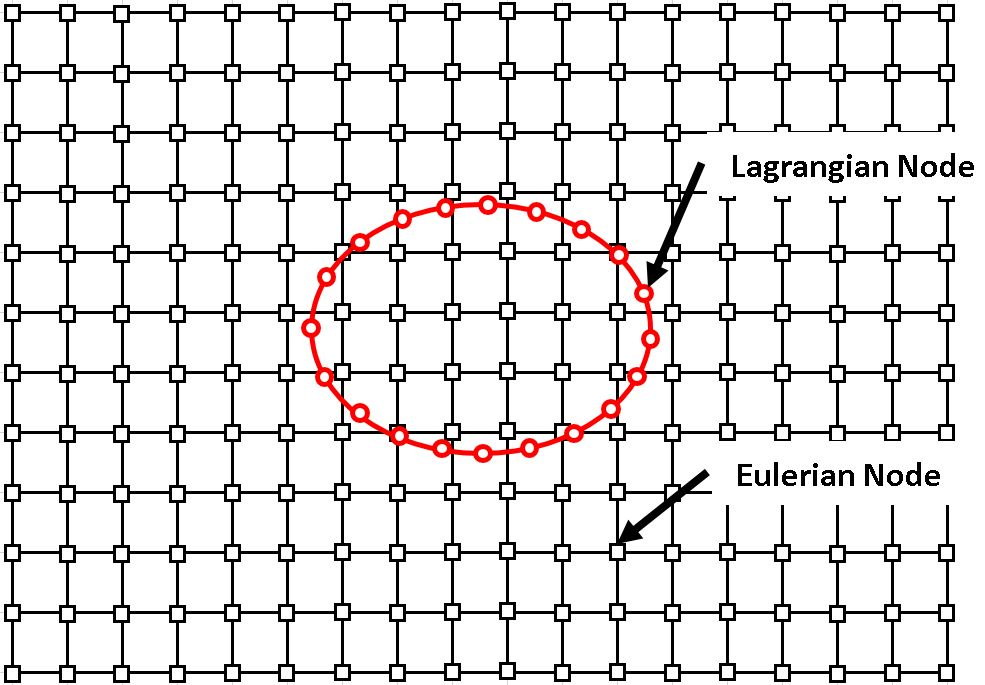
\includegraphics[height=5.0cm]{figure/immerdBoundary.jpg}
	\caption{Immersed boundary illustration}
	\label{fig:immersedBoundary}
\end{figure}
%
Shin et al. investigated the stability of the virtual boundary formulation for various types of regularized delta functions \cite{shin2008assessment}. These functions have different bandwidths which correspond to the number of Eulerian points where the effect of the forcing function is distributed; however; they are not continuously differentiable. In the continuum sensitivity analysis approach, the governing equations are differentiated to get the sensitivity equations. Therefore, it is required for the delta functions to have a continuous derivative. We propose the following Regularized Delta (RD) function formulation that satisfies this need.
%
\begin{equation}\label{eq:heavisideFunction}
	\delta_h(\mathbf{x}) = \frac{1}{h^3} \phi \left( \frac{x - x_k}{h} \right)
									 \phi \left( \frac{y - y_k}{h} \right)
									 \phi \left( \frac{z - z_k}{h} \right)
\end{equation}
%
where $h$ is the distance between the Eulerian nodes. $\phi$ is defined as:
%
\begin{equation}\label{eq:continuousDeltaFunction}
	\phi(r) = \dfrac{1}{\eta} \left( \dfrac{-\tanh^{2}{\left (\dfrac{r}{\eta} \right )} + 1}{2} \right)
	               \quad , \quad 
	               r = \frac{x - x_k}{h}
\end{equation}
%
For the RD function, the free parameter ($\eta$) is calculated by selecting how fast the RD function decays when moving further from its symmetry axis. The free parameter for the RD function is defined in Equation \eqref{eq:etaGuideForRDfunction}.
%
\begin{equation}\label{eq:etaGuideForRDfunction}
    \eta = \frac{R}{\tanh^{-1} (\sqrt{1 - p})}
\end{equation}
%
The RD function drops to $p$ percent of its value at the symmetry axis at a distance $R$. %For example, for the RD function value to drop 99 percent ($p = 0.99$) within 0.01 ($R = 0.01$) of the symmetry axis of the RD function, the $\eta$ value is calculated as $0.0033$ based on Equation \eqref{eq:etaGuideForRDfunction}.
%
\begin{figure}[H]
	\centering
	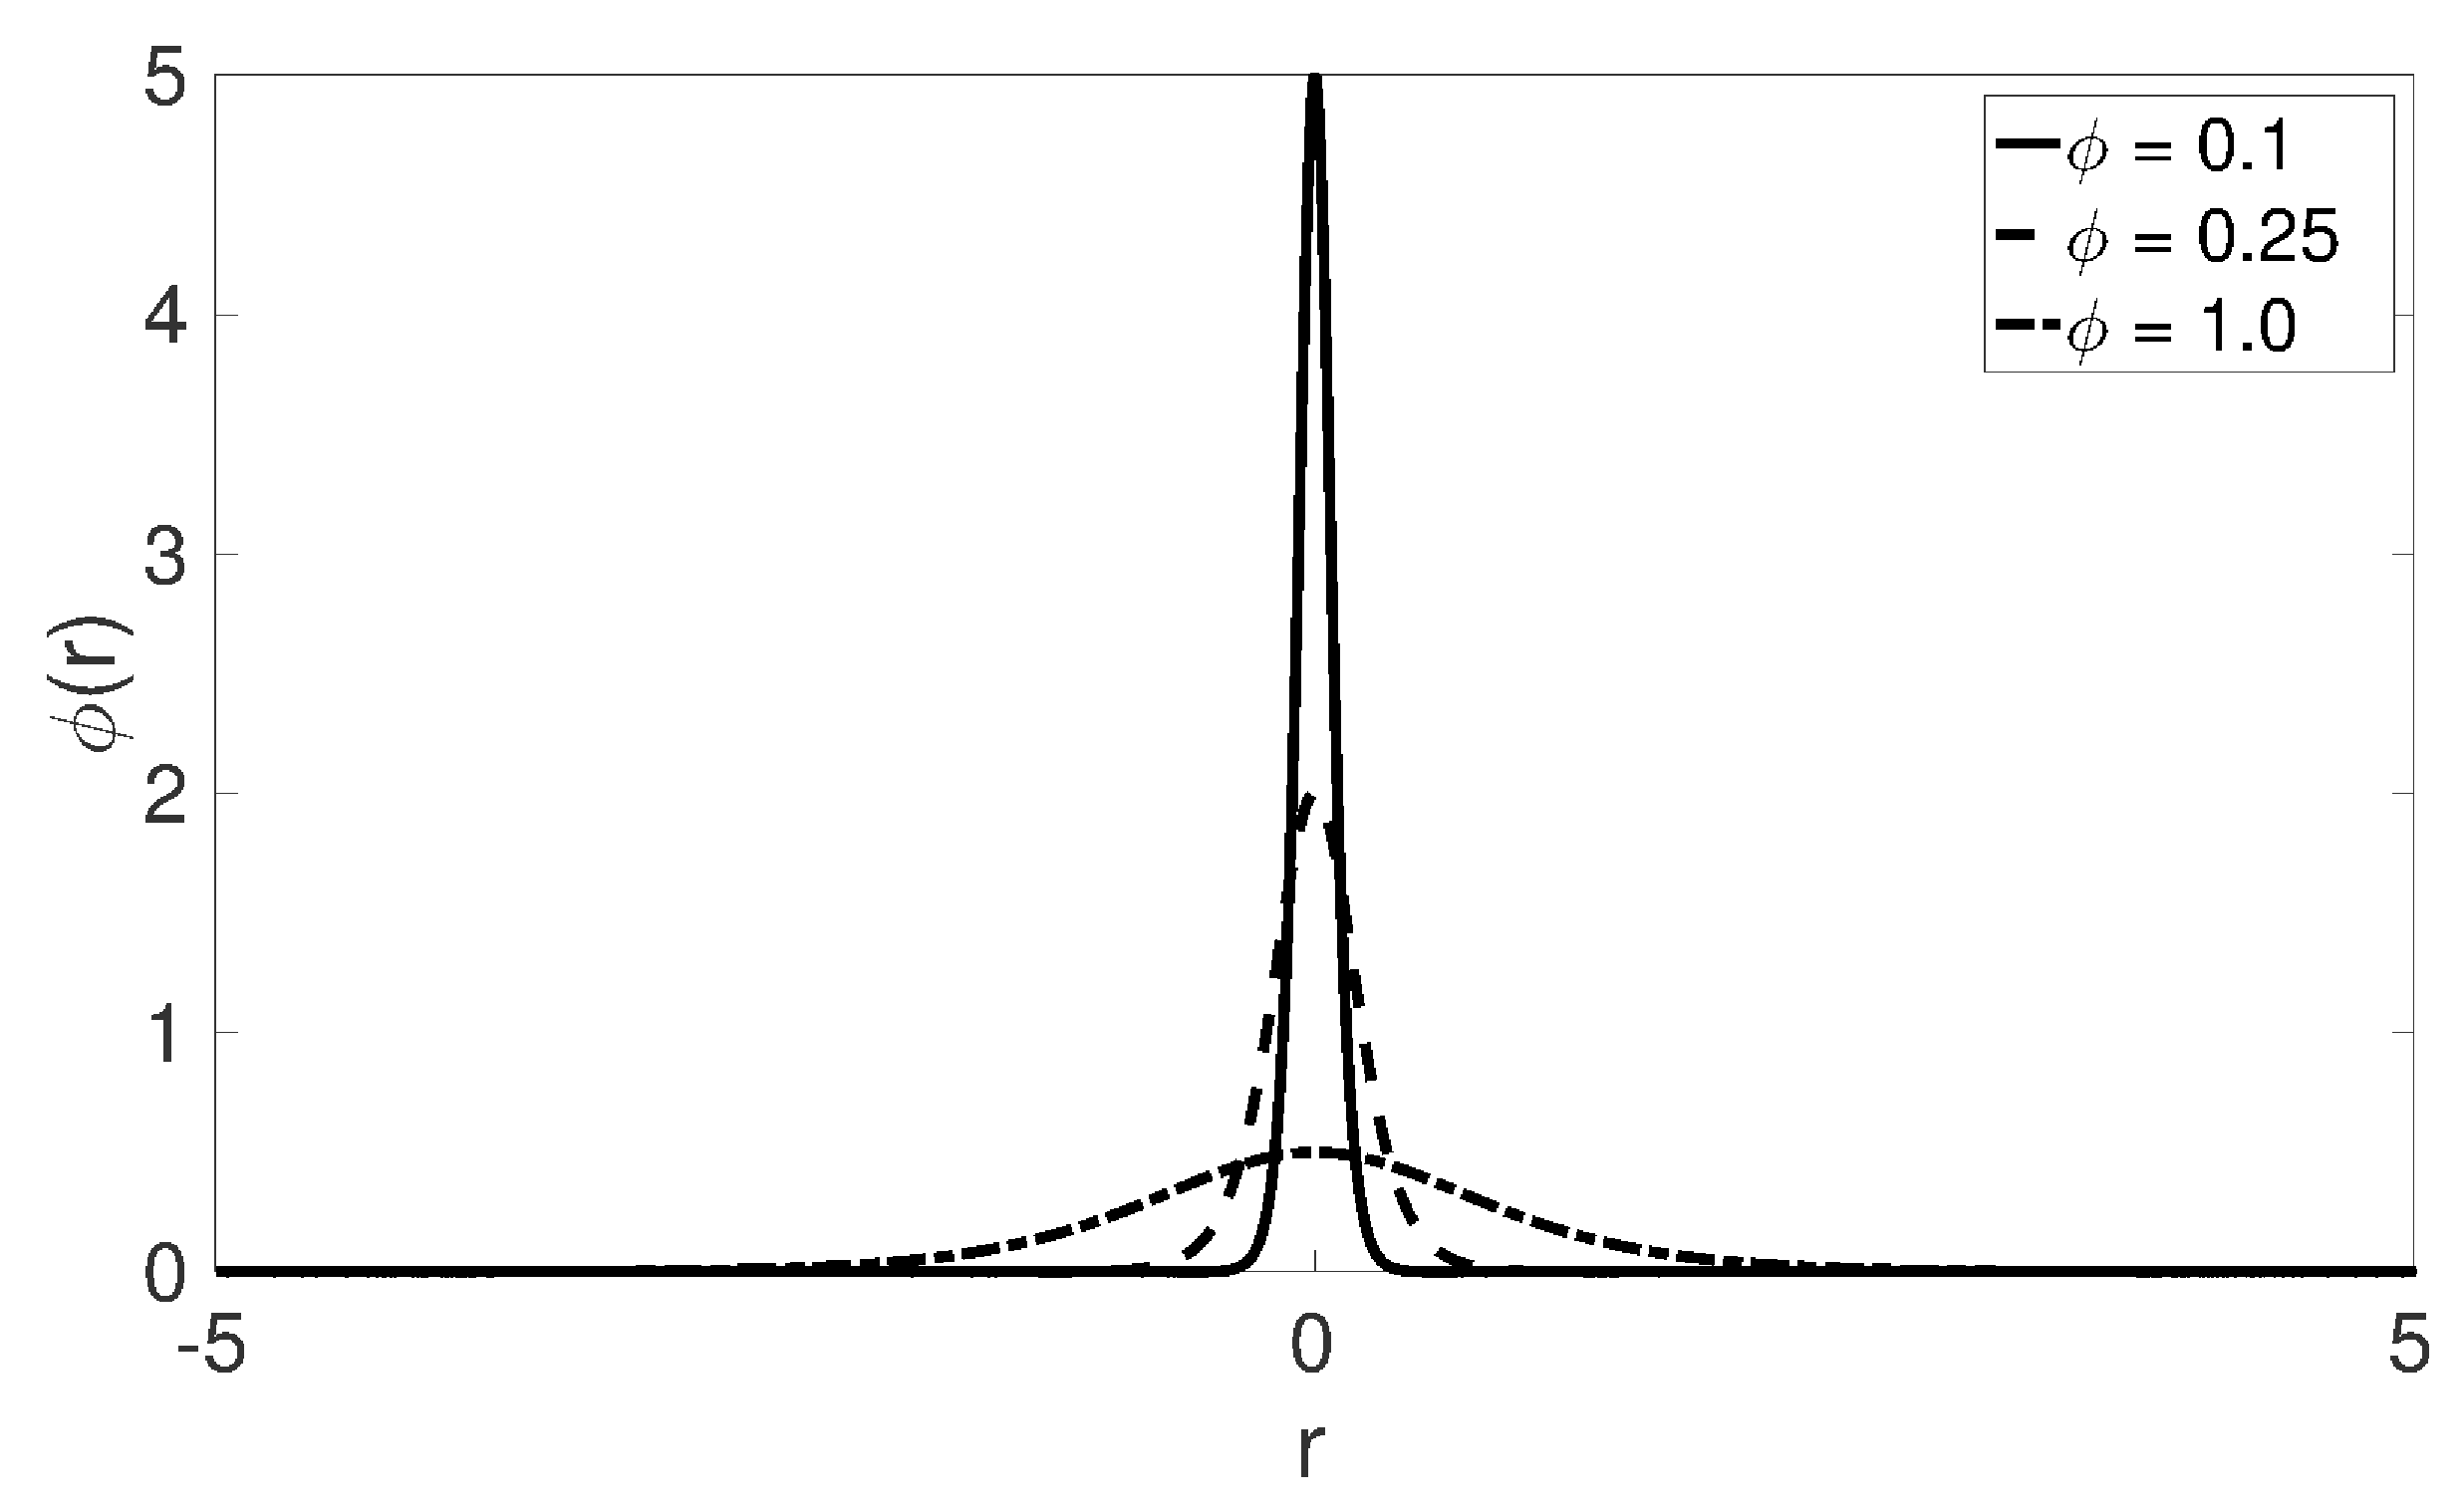
\includegraphics[height=5.0cm]{figure/heaviside_comparison.eps}
	\caption{Comparison between different delta function formulations.}
	\label{fig:heavisideComparison}
\end{figure}
%
Finally, the forcing function, $\mathbf{F}(\mathbf{x})$, can be written by combining equations \eqref{eq:forceAtEulerian}, \eqref{eq:forcingFunction}, and \eqref{eq:velocityAtLagrangian}.
%
\begin{equation}
\begin{aligned}\label{eq:forceAtEulerianFinal}
	\mathbf{f}^f(\mathbf{x}, t) = 
	\int_\Omega 
	&\left\{
 	\alpha \int_0^t
	\left[
	\int_\Omega \mathbf{u}^f (\mathbf{x}, t) \delta(\mathbf{x} - \mathbf{x}_k) d\mathbf{x} - \mathbf{U}\left( \mathbf{x}_k, t \right)
	\right]dt + \right. \\
	&\left.
	\beta \left[
	\int_\Omega \mathbf{u}^f (\mathbf{x}, t) \delta(\mathbf{x} - \mathbf{x}_k) d\mathbf{x} - \mathbf{U}\left( \mathbf{x}_k, t \right)
	\right]
	\right\} \delta(\mathbf{x} - \mathbf{x}_k) d\mathbf{x}_k
\end{aligned}
\end{equation}
%
In Equation \eqref{eq:forceAtEulerianFinal}, the integrals on the domain, $\Omega$, transfer the data between the Lagrangian and Eulerian domains. The inner integrals map the velocities from Eulerian to Lagrangian nodes to calculate the forces at the Lagrangian nodes, $\mathbf{f}\left( \mathbf{x}, t \right)$. The outer integral maps the forcing function from the Lagrangian to Eulerian nodes where the governing equations are solved (Figure \ref{fig:mappingDataE2L}).
%
\begin{figure}[H]
	\centering
	\subfigure[Velocity calculation at the Lagrangian nodes.]
	{
	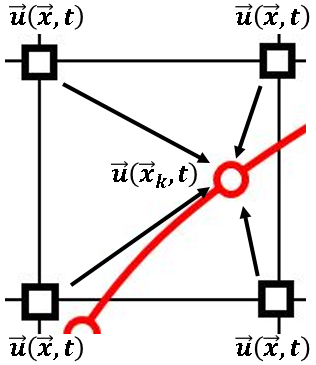
\includegraphics[height=5.5cm]{figure/mapping_1.png}
	}
	\quad
	\subfigure[Forcing function evaluation.]
	{
	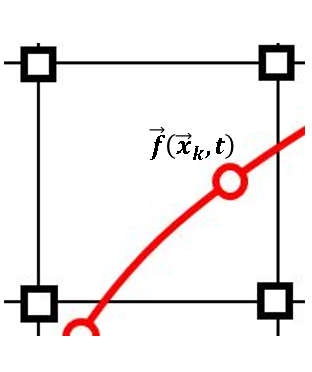
\includegraphics[height=5.5cm]{figure/mapping_2.png}
	}
	\quad
	\subfigure[Forcing function transfer to the Eulerian nodes.]
	{
	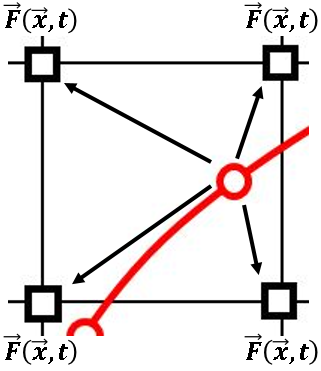
\includegraphics[height=5.5cm]{figure/mapping_3.png}
	}
	\caption{Data transfer between Eulerian and Lagrangian nodes.}
	\label{fig:mappingDataE2L}
\end{figure}
%
% -.-.-.-.-.-.-.-.-.-.-.-.-.-.-.-.-.-.-.-.-.-.-.-.-.-.-.-.-.-.-.-.-.-.-.-.-.-.-.-.-.-.-.-.-
\subsection{Multidisciplinary Shape Sensitivity Analysis}\label{sec:SA}
It is beneficial to first formulate the sensitivity equations in the general form. Figure \ref{fig:domain} represents the domain, $\Omega$, in the Cartesian space. This domain is the union of the solid, $\Omega_s$, and fluid, $\Omega_f$, domains where the Navier-Stokes equations are solved. The far field boundary conditions which are defined on the sides of this domain, $\Gamma$, are not affected by the design variables. By using this approach, the boundaries of the solid domain are added to the fluid's governing equations as mentioned in the previous section.
%
\begin{figure}[H]
	\centering
	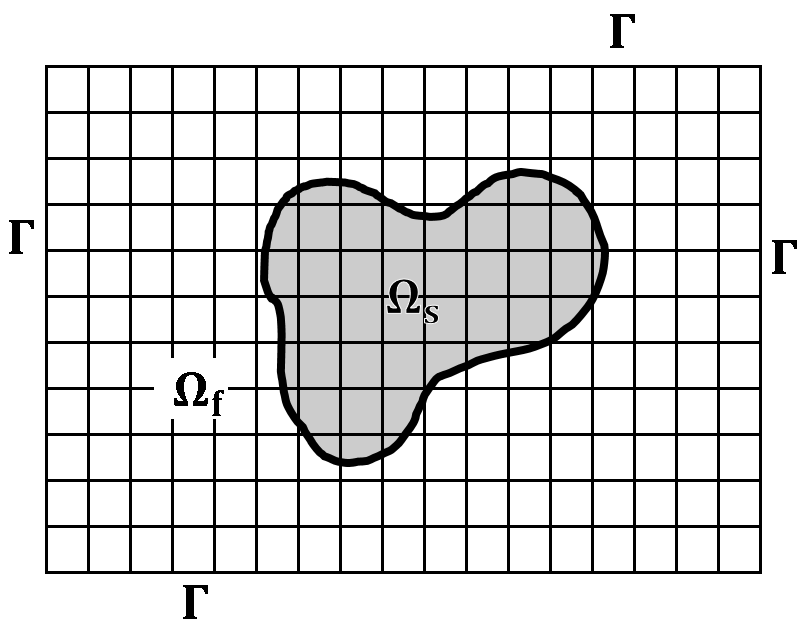
\includegraphics[height=5.0cm]{figure/domain.jpg}
	\caption{Computational domain, $\Omega = \Omega_f \cup \Omega_s$, with boundary of $\Gamma$}
	\label{fig:domain}
\end{figure}
%
The governing equation and boundary conditions are written in the general form as:
%
\begin{subequations}\label{eq:generalFormForGE}
\begin{equation}
	A(\mathbf{u}, \mathbf{b}) = f(\mathbf{x}, t, \mathbf{b}) \quad \text{on} \quad \Omega
\end{equation}
\begin{equation}
	B(\mathbf{u}, \mathbf{b}) = g(\mathbf{x}, t, \mathbf{b}) \quad \text{on} \quad \Gamma
\end{equation}
\end{subequations}
%
Here, $A$ and $B$ are the differential operators for the governing equations and boundary conditions, respectively. $\mathbf{u}$ is the vector of response variables that could be displacements in structural mechanics or velocities and pressures in fluid dynamics. The vectors $\mathbf{x}$ and $\mathbf{b}$ contain spatial coordinates and design variables, respectively. The total sensitivity of the response variable $\mathbf{u}$ to the $i^\text{th}$ design variable $b_i$ is calculated as:
%
\begin{equation}
	\frac{D\mathbf{u}}{Db_i	} = \frac{\partial \mathbf{u}}{\partial b_i} + 
	                        \frac{\partial \mathbf{u}}{\partial \mathbf{x}} \cdot \frac{\partial \mathbf{x}}{\partial b_i}
\end{equation}
%
This material derivative consists of the local design derivative, $\partial \mathbf{u} / \partial b_i$, plus a convective term, $\partial \mathbf{u} / \partial \mathbf{x} \cdot \partial \mathbf{x} / \partial b_i$. The local design derivative is a measure of how much the response at a point alters due to change in the design parameters. The convective term tracks the movement of the material point when the spatial coordinates change with the design variable. The geometric domain can be a function of the design variables in the case of body conformal meshes (Figure \ref{fig:conformalVSnonconformal}). However, non-body conformal meshes will not change as the design parameter varies. Therefore, the convective term is equal to zero \cite{gobal2014continuum}. Thus, the local and total forms of the sensitivities are equal.
%
\begin{subequations}\label{eq:C5_fluidSA}
\begin{align}
	&\rho^f \frac{\partial}{\partial t} \left( \frac{\partial \mathbf{u}^f}{\partial b} \right) + 
	\rho^f \frac{\partial \mathbf{u}^f}{\partial b} \cdot \nabla \mathbf{u}^f +
	\rho^f \mathbf{u}^f \cdot \nabla \left( \frac{\partial \mathbf{u}^f}{\partial b} \right) = 
	\nabla \cdot \left( \frac{\partial \mathbf{\sigma}^f}{\partial b} \right) +
	\rho^f \frac{\partial \mathbf{f}^f}{\partial b}
	\\
	&\nabla \cdot \left( \frac{\partial \mathbf{u}^f}{\partial b} \right) = 0
	\\
	&\frac{\partial \mathbf{\sigma}^f}{\partial b} = 
	\mu \left[ \nabla \left( \frac{\partial \mathbf{u}^f}{\partial b} \right) + 
	           \nabla \left( \frac{\partial \mathbf{u}^f}{\partial b} \right)^T \right] - 
	\frac{\partial p^f}{\partial b} \mathbf{I}
\end{align}
\end{subequations}
%
The effect of solid boundary shape sensitivity is introduced in Equation \eqref{eq:C5_fluidSA} through $\partial \mathbf{f}^f / \partial b$, more specifically through the derivative of the regularized delta function with respect to design variable, $b_i$. The derivative of the forcing function is derived as
%
\begin{equation}
\begin{aligned}\label{eq:forceingFunctionDerivative}
	\frac{\partial \mathbf{f}^f}{\partial b}(\mathbf{x}, t) = 
	\int_\Omega 
	&\left\{
 	\alpha \int_0^t
	\left[
	\int_\Omega \mathbf{u^\prime} (\mathbf{x}, t) \delta(\mathbf{x} - \mathbf{x}_k) d\mathbf{x} - 
	\int_\Omega \mathbf{u} (\mathbf{x}, t) \frac{\partial \delta(\mathbf{x} - \mathbf{x}_k)}{\partial \mathbf{x}_k} \frac{\partial \mathbf{x}_k}{\partial b_i} d\mathbf{x}
	\right]dt + \right. \\
	&\left.
	\quad \beta
	\left[
	\int_\Omega \mathbf{u^\prime} (\mathbf{x}, t) \delta(\mathbf{x} - \mathbf{x}_k) d\mathbf{x} - 
	\int_\Omega \mathbf{u} (\mathbf{x}, t) \frac{\partial \delta(\mathbf{x} - \mathbf{x}_k)}{\partial \mathbf{x}_k} \frac{\partial \mathbf{x}_k}{\partial b_i} d\mathbf{x}
	\right]
	\right\} \delta(\mathbf{x} - \mathbf{x}_k) d\mathbf{x}_k + \\
	\int_\Omega 
	&\left\{
 	\alpha \int_0^t
	\left[
	\int_\Omega \mathbf{u} (\mathbf{x}, t) \delta(\mathbf{x} - \mathbf{x}_k) d\mathbf{x} - \mathbf{U}\left( \mathbf{x}_k, t \right)
	\right]dt + \right. \\
	&\left.
	\quad \beta \left[
	\int_\Omega \mathbf{u} (\mathbf{x}, t) \delta(\mathbf{x} - \mathbf{x}_k) d\mathbf{x} - \mathbf{U}\left( \mathbf{x}_k, t \right)
	\right]
	\right\} \frac{\partial \delta(\mathbf{x} - \mathbf{x}_k)}{\partial \mathbf{x}_k} \frac{\partial \mathbf{x}_k}{\partial b_i} d\mathbf{x}_k
\end{aligned}
\end{equation}
%
where $\mathbf{u^\prime}\left( \mathbf{x}, t \right)$ is the sensitivity of the velocity to design parameter, $b_i$. The chain rule was used to differentiate the regularized delta function with the design variable, $b_i$. The shape of the design variable only affects the location of the Lagrangian points. The derivative of the Lagrangian nodes, $\mathbf{x}_k$, with respect to $b_i$ can be easily calculated by the problem definition since the dependency of the shape of the domain (Lagrangian nodes), and design variables are known. The derivative of the regularized delta function to the Lagrangian node, $x_k$, is calculated analytically by differentiating Equation \eqref{eq:continuousDeltaFunction}. This results in a system of differential equations for the sensitivity response of the system. This method has a significant advantage over the conventional body conforming approaches since there is no need to calculate the sensitivity of the boundary condition or computational mesh with respect to the design variable.
% -.-.-.-.-.-.-.-.-.-.-.-.-.-.-.-.-.-.-.-.-.-.-.-.-.-.-.-.-.-.-.-.-.-.-.-.-.-.-.-.-.-.-.-.-
\subsection{Shape Parameterization}\label{sec:shapeParameterization}
There are many techniques available to parametrize the shape for design optimization. Some of the techniques have more advantage in terms of the convergence rate and the range of the shape they can represent. However, every parameterization method must have the following characteristics \cite{salunke2014airfoil}: i) it should minimize the total degrees of freedom, ii) it should be able to represent a wide variety of shapes, and iii) parameters should be simple to formulate and impose.

Bezier curve is one of the popular parametrization techniques to represent airfoils. A Bezier curve of degree \emph{n} is controlled by \emph{n+1} control points in a plane. Shape functions of the Bezier curve are known as Bernstein polynomials and are defined as
%
\begin{equation}\label{eq:bernsteinPolynomials}
	B_i^n(t) = {n \choose i} (1 - t)^{n - i} t^i
\end{equation}
%
where $t$ varies between $0$ and $1$. The Bezier curve, $C(t)$, associated the control points, $P_i$, is defined as
%
\begin{equation}\label{eq:bezierCurve}
	C(t) = \sum_{i=0}^n P_i B_i^n(t)
\end{equation}
%
We parametrized the NACA 0012 and RAE 2822 airfoils with four and five control points respectively. This is shown in Figure \ref{fig:airfoilParameterization}. The control points are shown as crosses and circles. The control points indicated by the circles on the top and bottom surface of the airfoil are used as design variables. The shape sensitivity of the parametrized airfoils to design variable is calculated by analytical differentiating Equation \eqref{eq:bezierCurve} with respect to the corresponding control point. This information is fed to the differentiated Navier-Stokes equations to calculate the shape sensitivities.
%
\begin{figure}[H]
	\centering
	\subfigure[NACA 0012 airfoil]
	{
	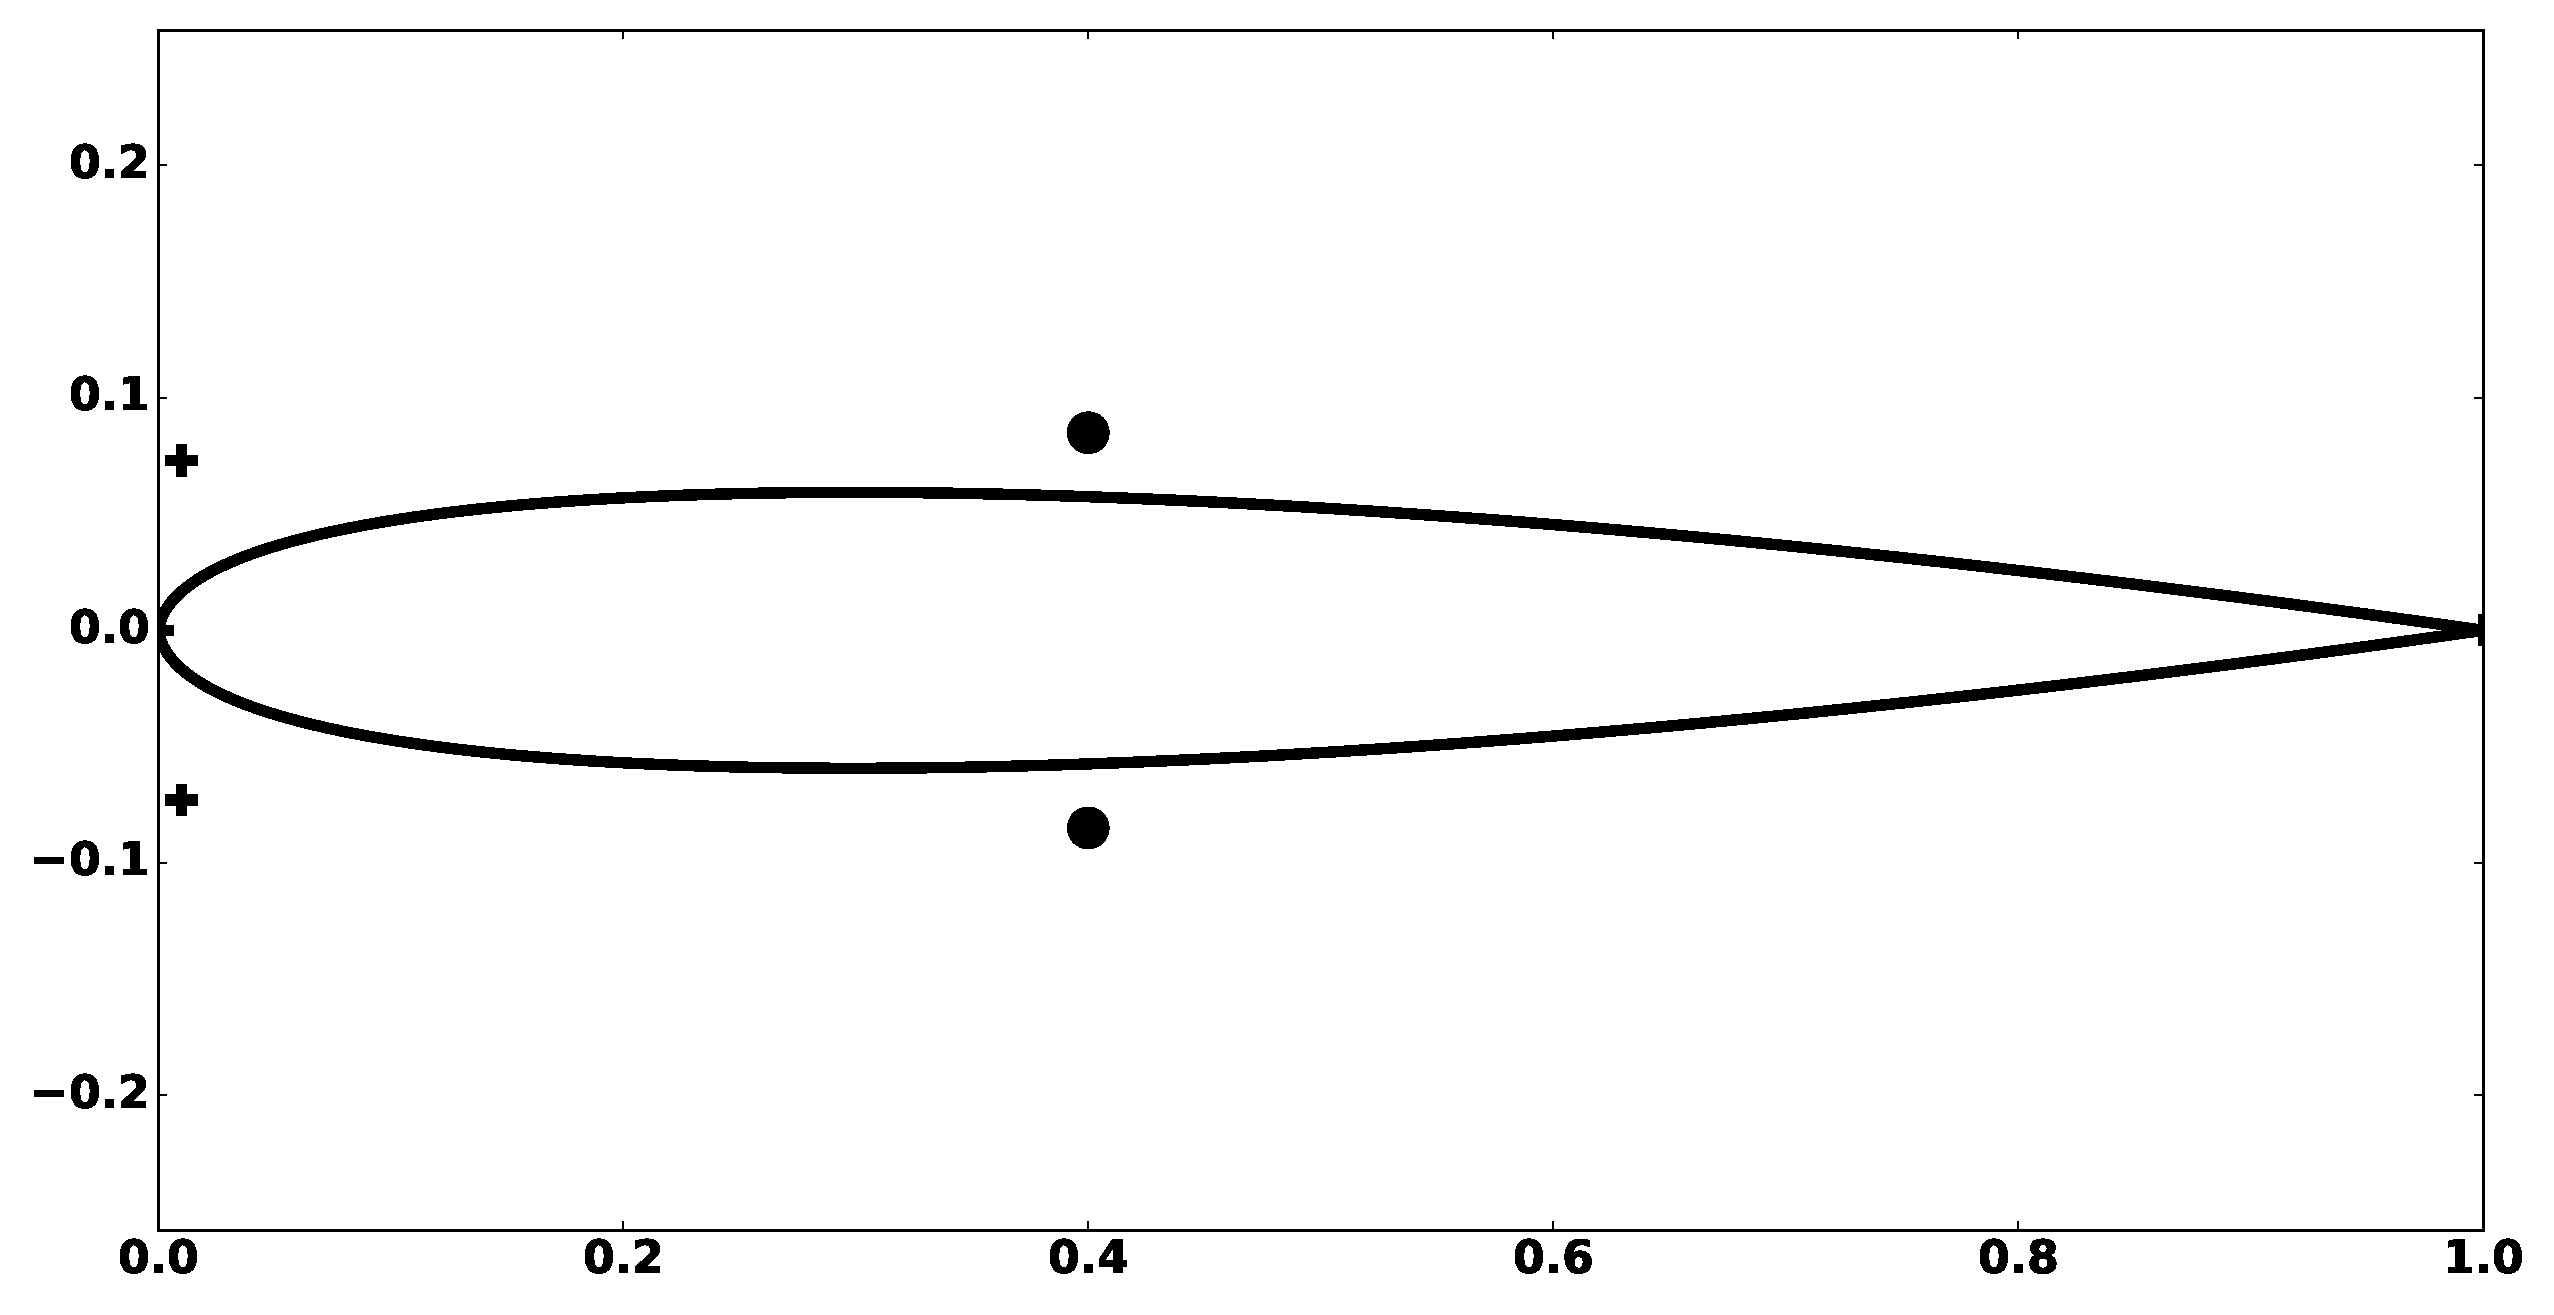
\includegraphics[height=3.75cm]{figure/NACA0012.eps}
	}
	\quad
	\subfigure[RAE 2822 airfoil]
	{
	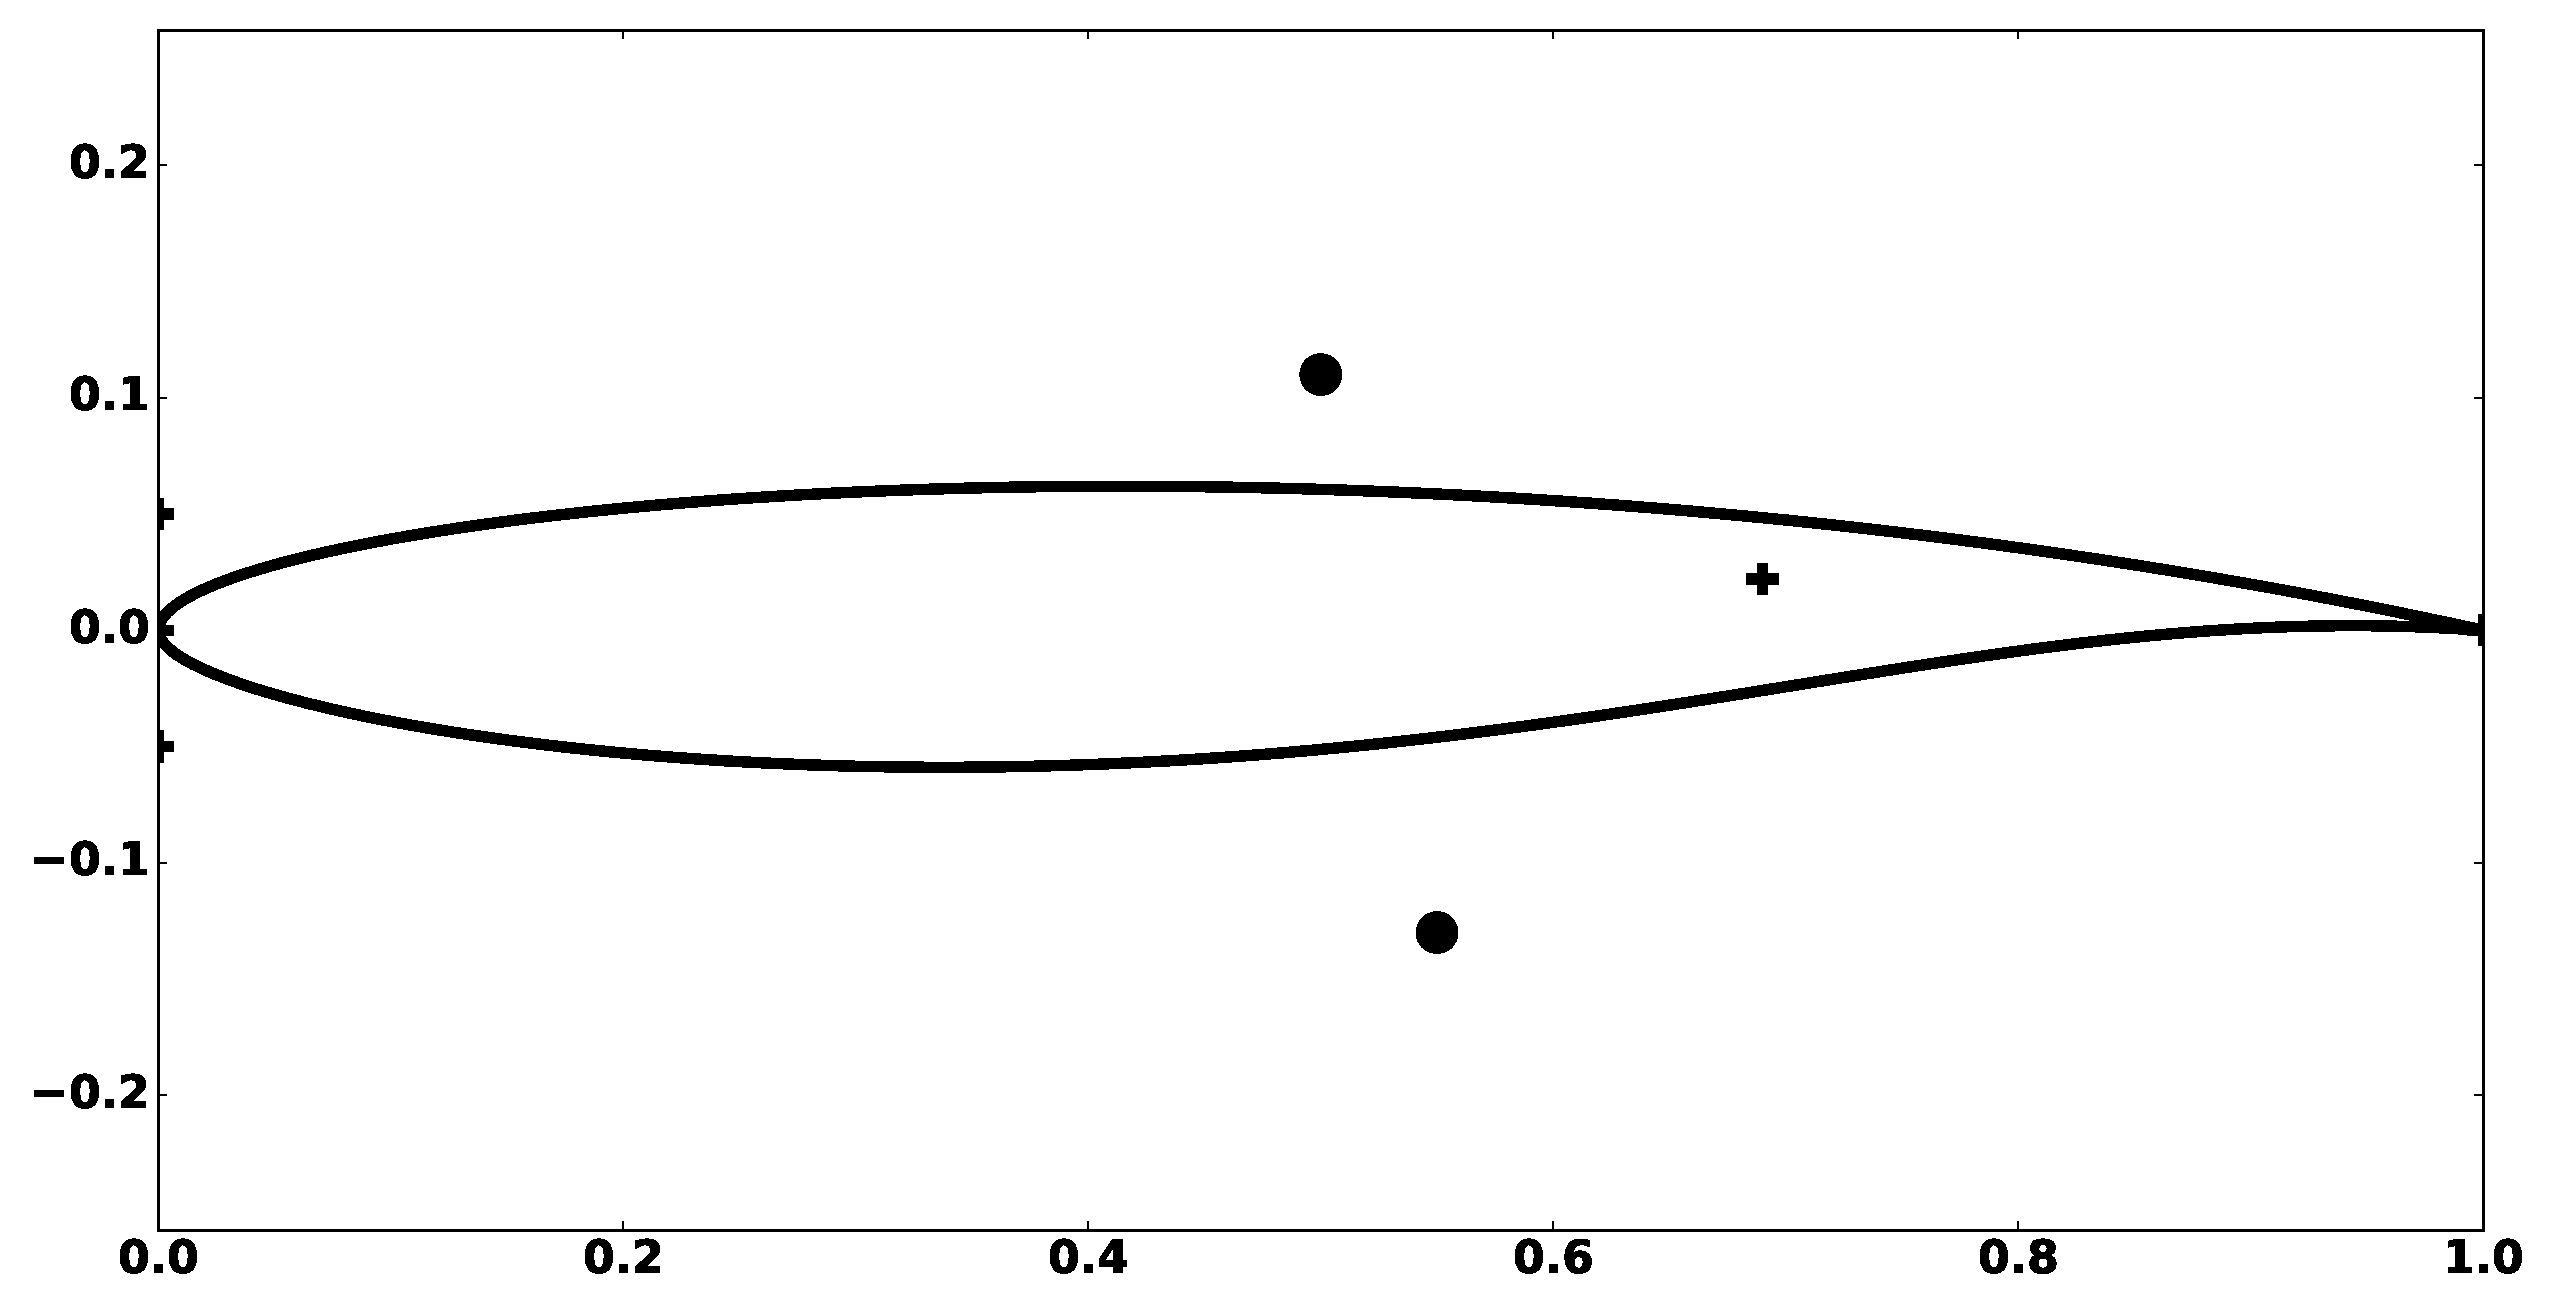
\includegraphics[height=3.75cm]{figure/RAE2822.eps}
	}
	\caption{Shape representation using Bezier curves. Control points are shown with circles and crosses where circles represent the control points acting as shape design variables.}
	\label{fig:airfoilParameterization}
\end{figure}
%
% ==========================================================================================
\section{Priliminary Results}
Flow over two different airfoils is modeled using the immersed boundary approach. The governing equation is selected as the incompressible Navier-Stokes equations for this demonstration case with Reynolds number equal to $6.5 \times 10^6$. The final paper will include the compressible flow results for the immersed boundary formulation verified with the FUN3D flow solver. The domain shape and dimension is shown in Figure \ref{fig:physicalDomain}. 
%
\begin{figure}[H]
	\label{fig:physicalDomain}
\end{figure}
%
The airfoil shape is defined using 100 Lagrangian points for both cases. The sensitivity of surface pressure with respect to all shape design variables for two airfoils are shown in Figures \ref{fig:NACA0012sensitivity} and \ref{fig:RAE2822sensitivity} respectively. These results show a good comparison with the complex step results.
%
\begin{figure}[H]
	\centering
	\subfigure[Sensitivity to top surface shape change]
	{
	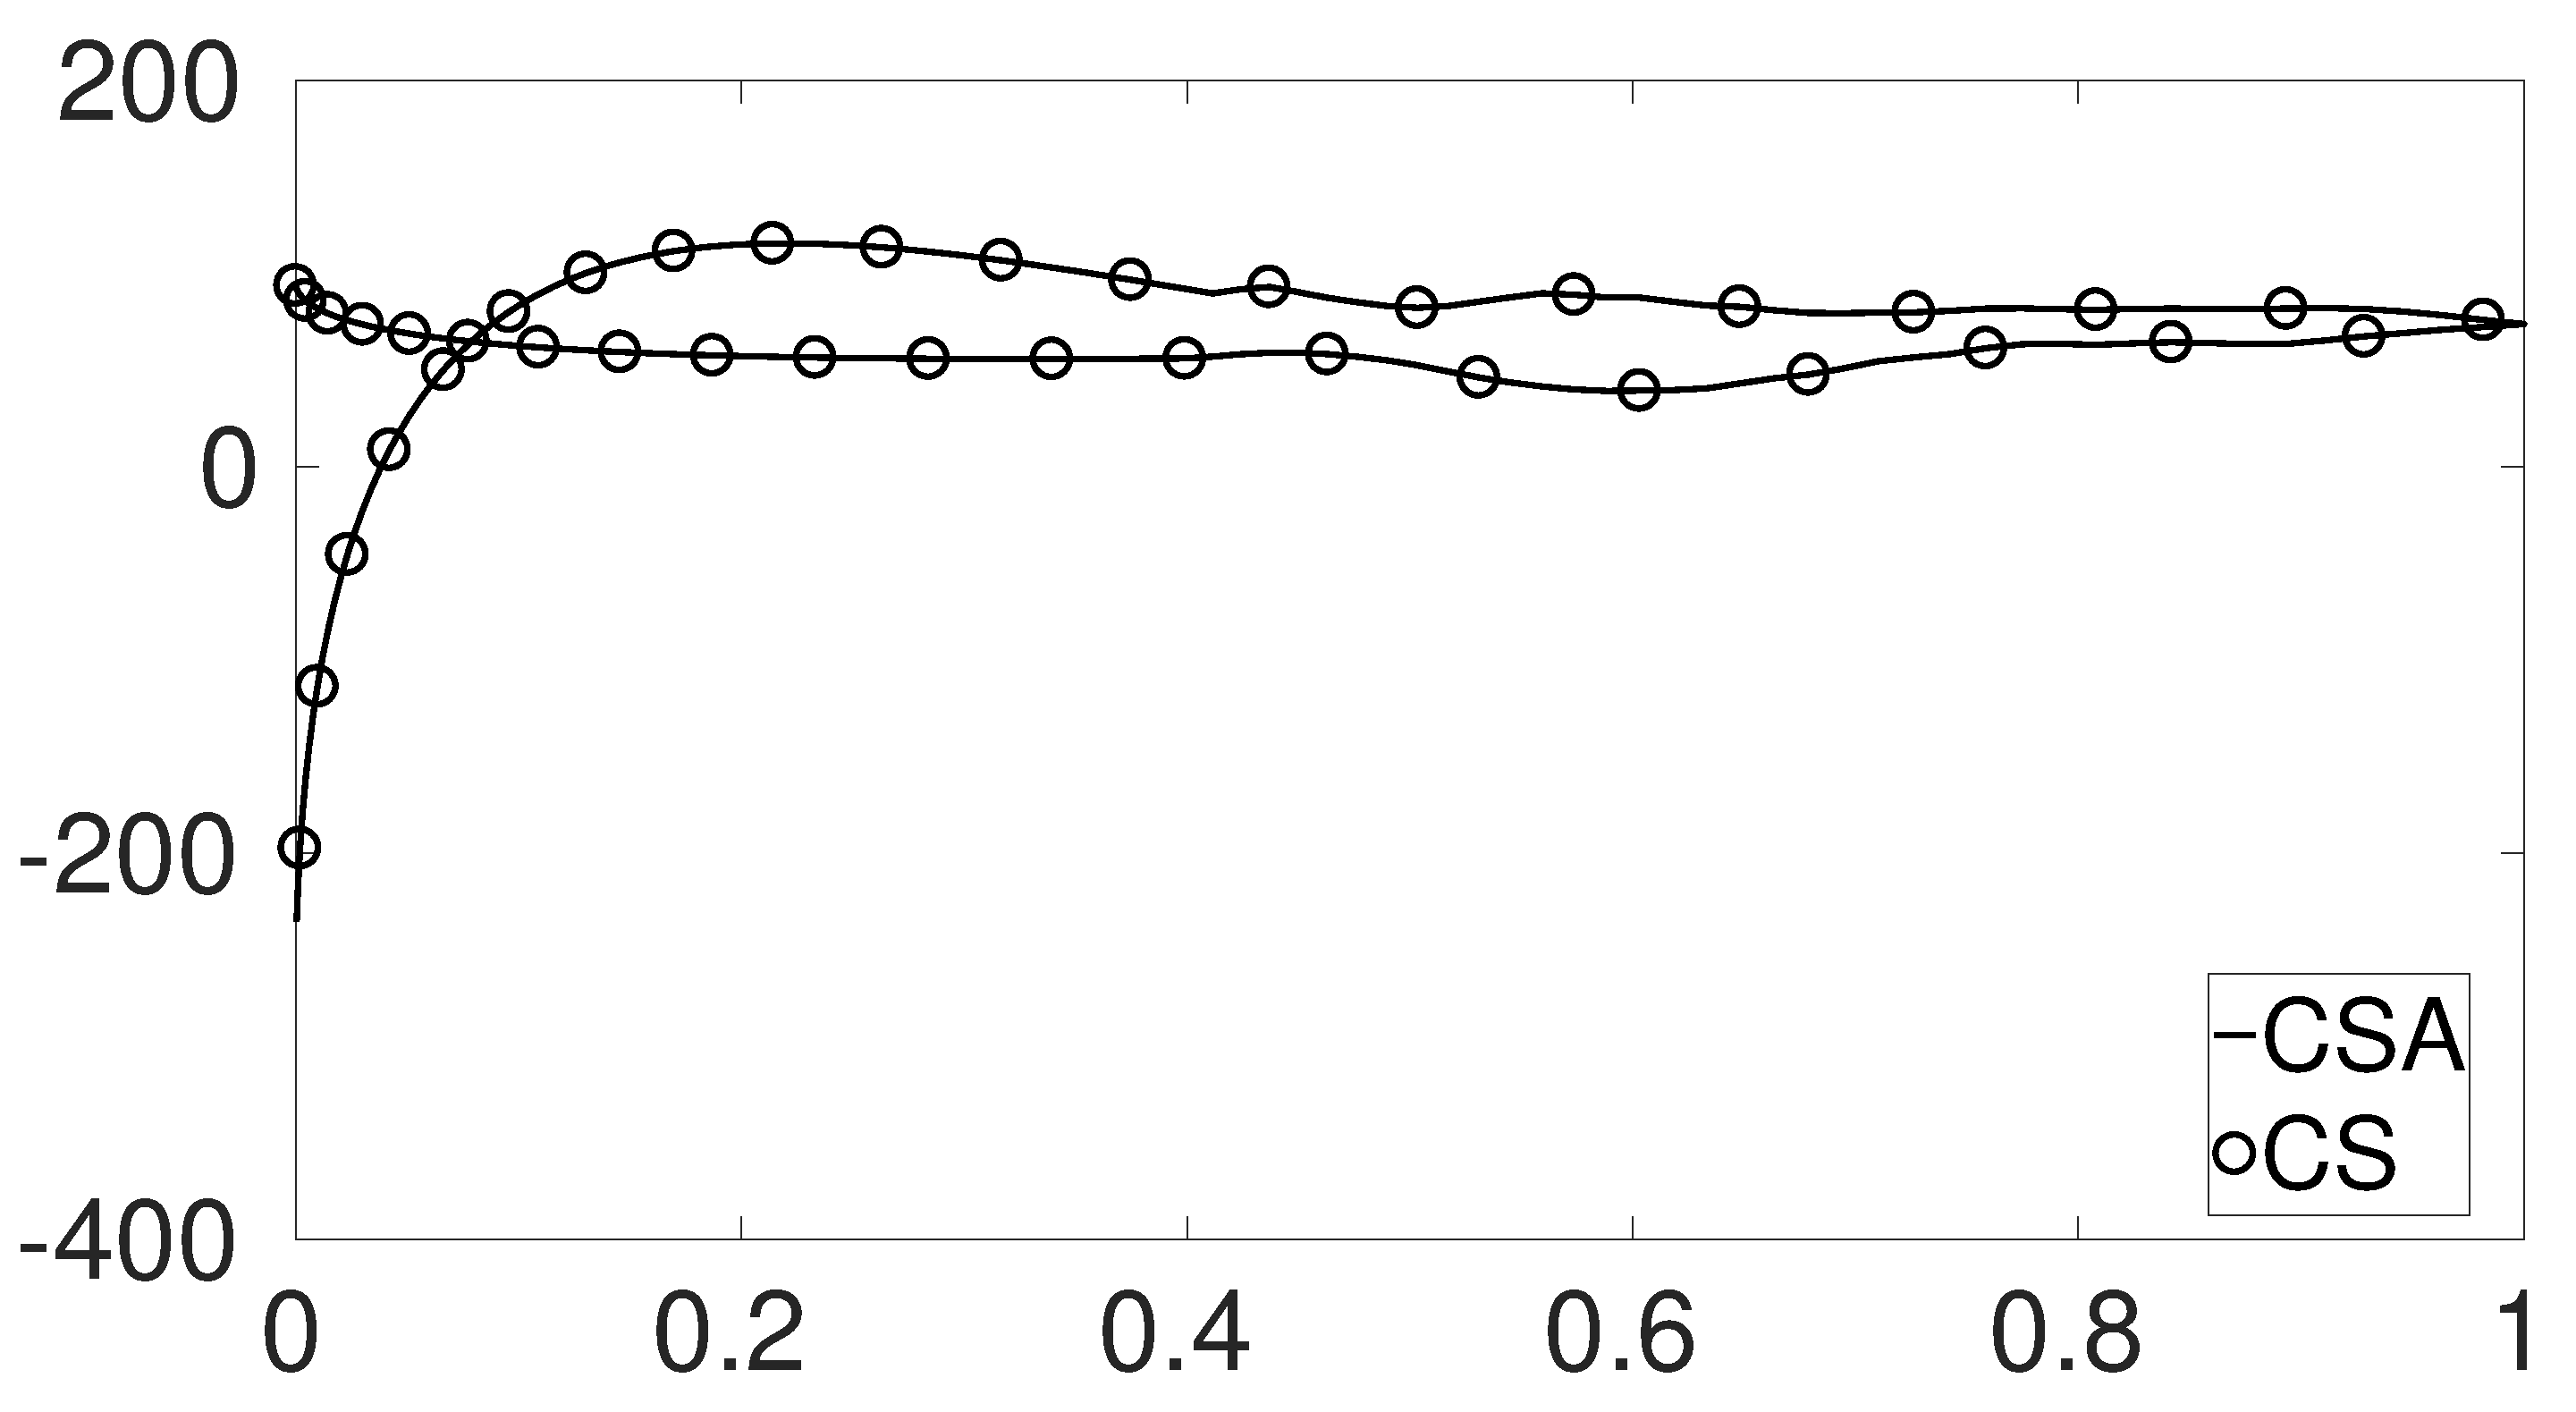
\includegraphics[height=4.0cm]{figure/NACA0012/sensitivity_NACA0012_topDV.eps}
	}
	\quad
	\subfigure[Sensitivity to bottom surface shape change]
	{
	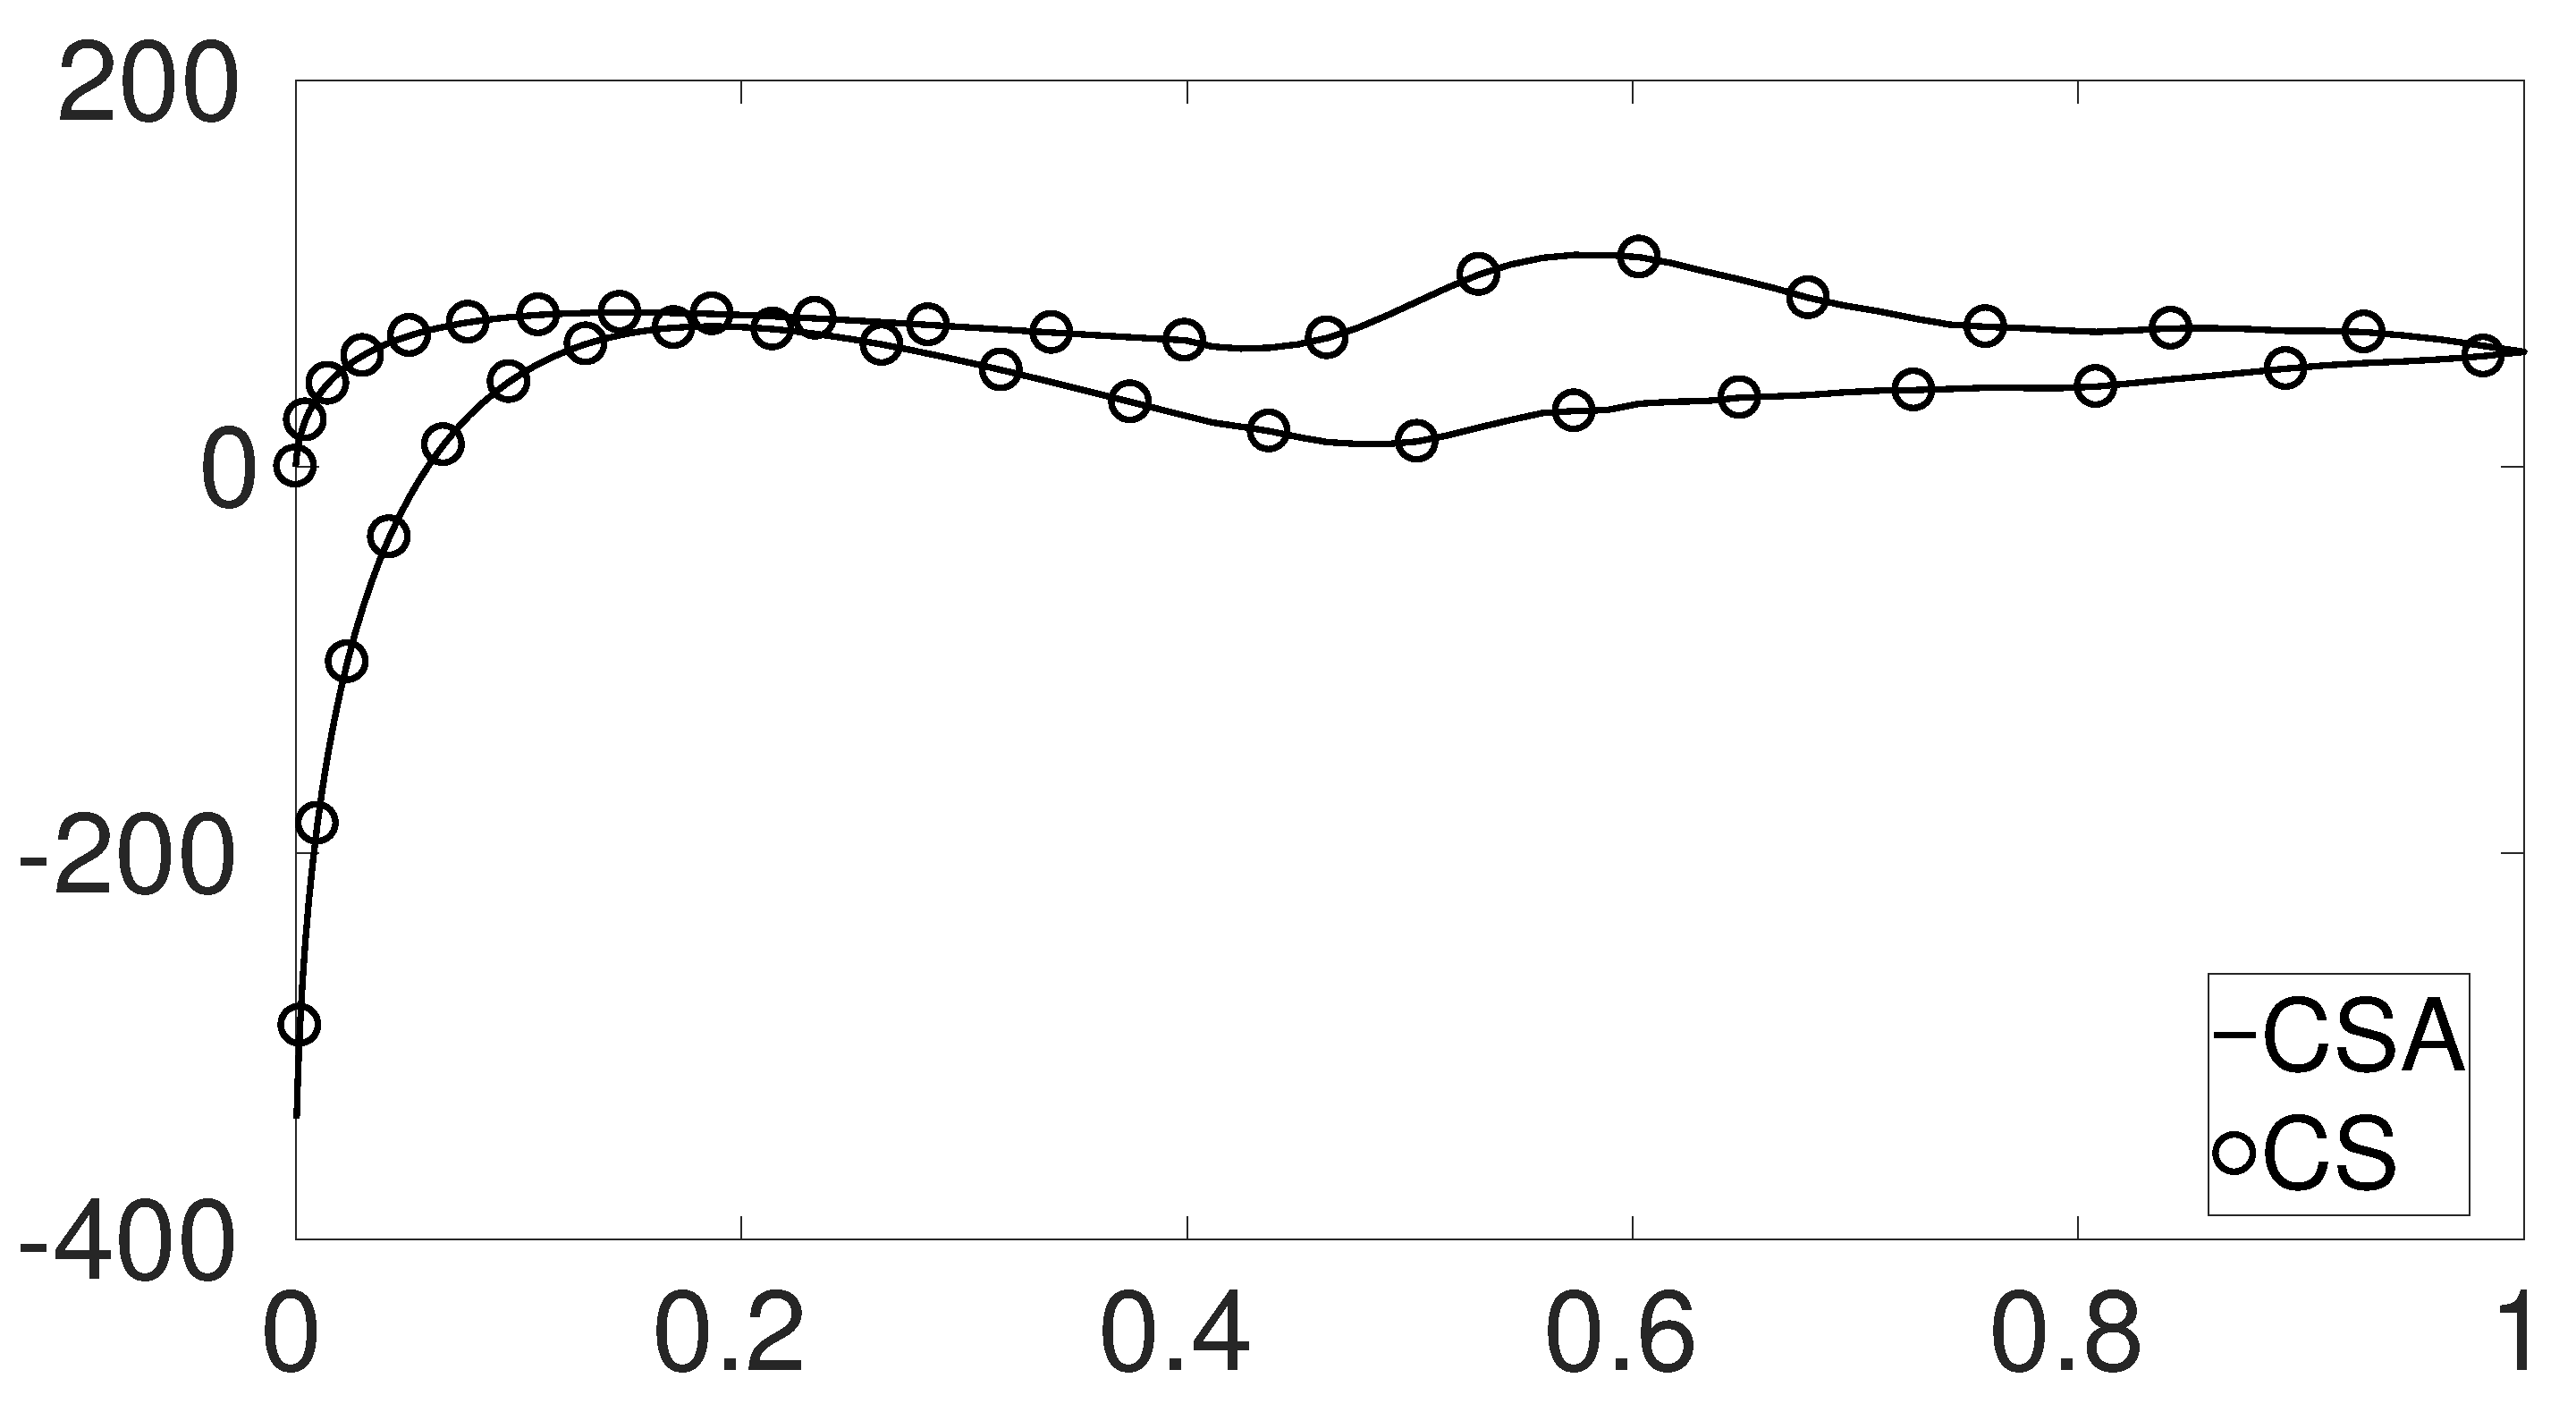
\includegraphics[height=4.0cm]{figure/NACA0012/sensitivity_NACA0012_bottomDV.eps}
	}
	\caption{NACA 0012 surface pressure shape sensitity results.}
	\label{fig:NACA0012sensitivity}
\end{figure}
%
%
\begin{figure}[H]
	\centering
	\subfigure[Sensitivity to top surface shape change]
	{
	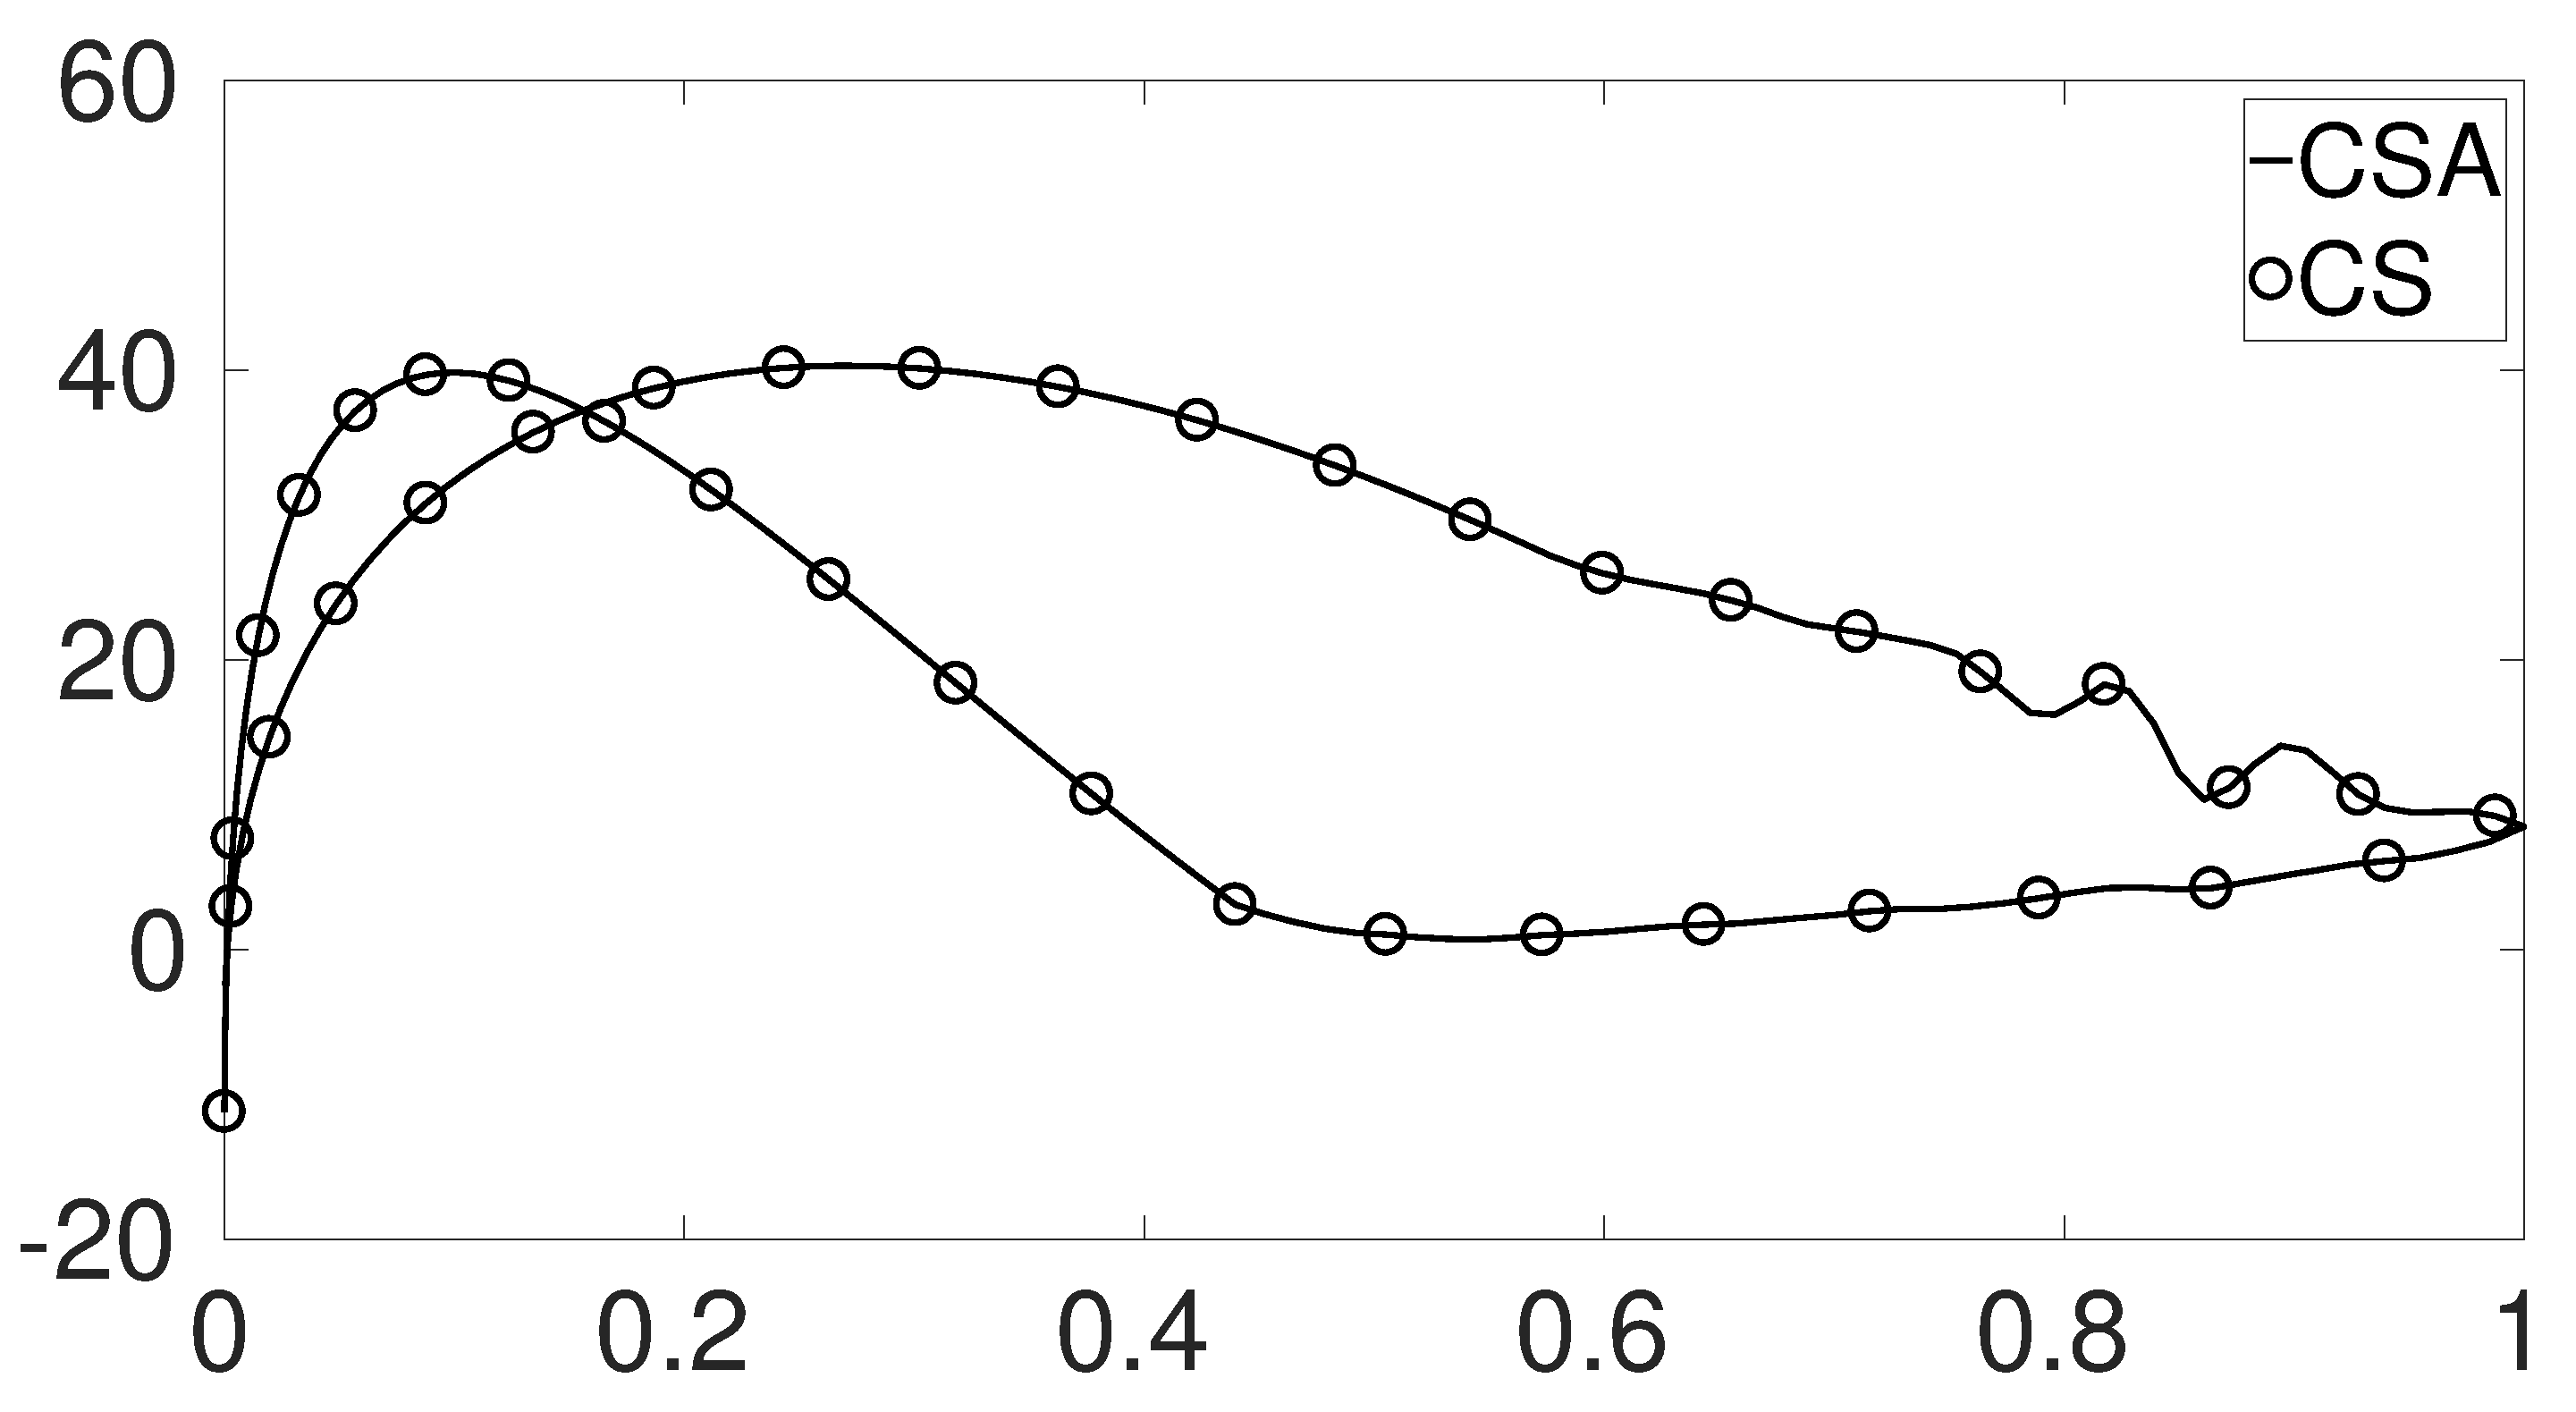
\includegraphics[height=4.0cm]{figure/RAE2822/sensitivity_RAE2822_topDV.eps}
	}
	\quad
	\subfigure[Sensitivity to bottom surface shape change]
	{
	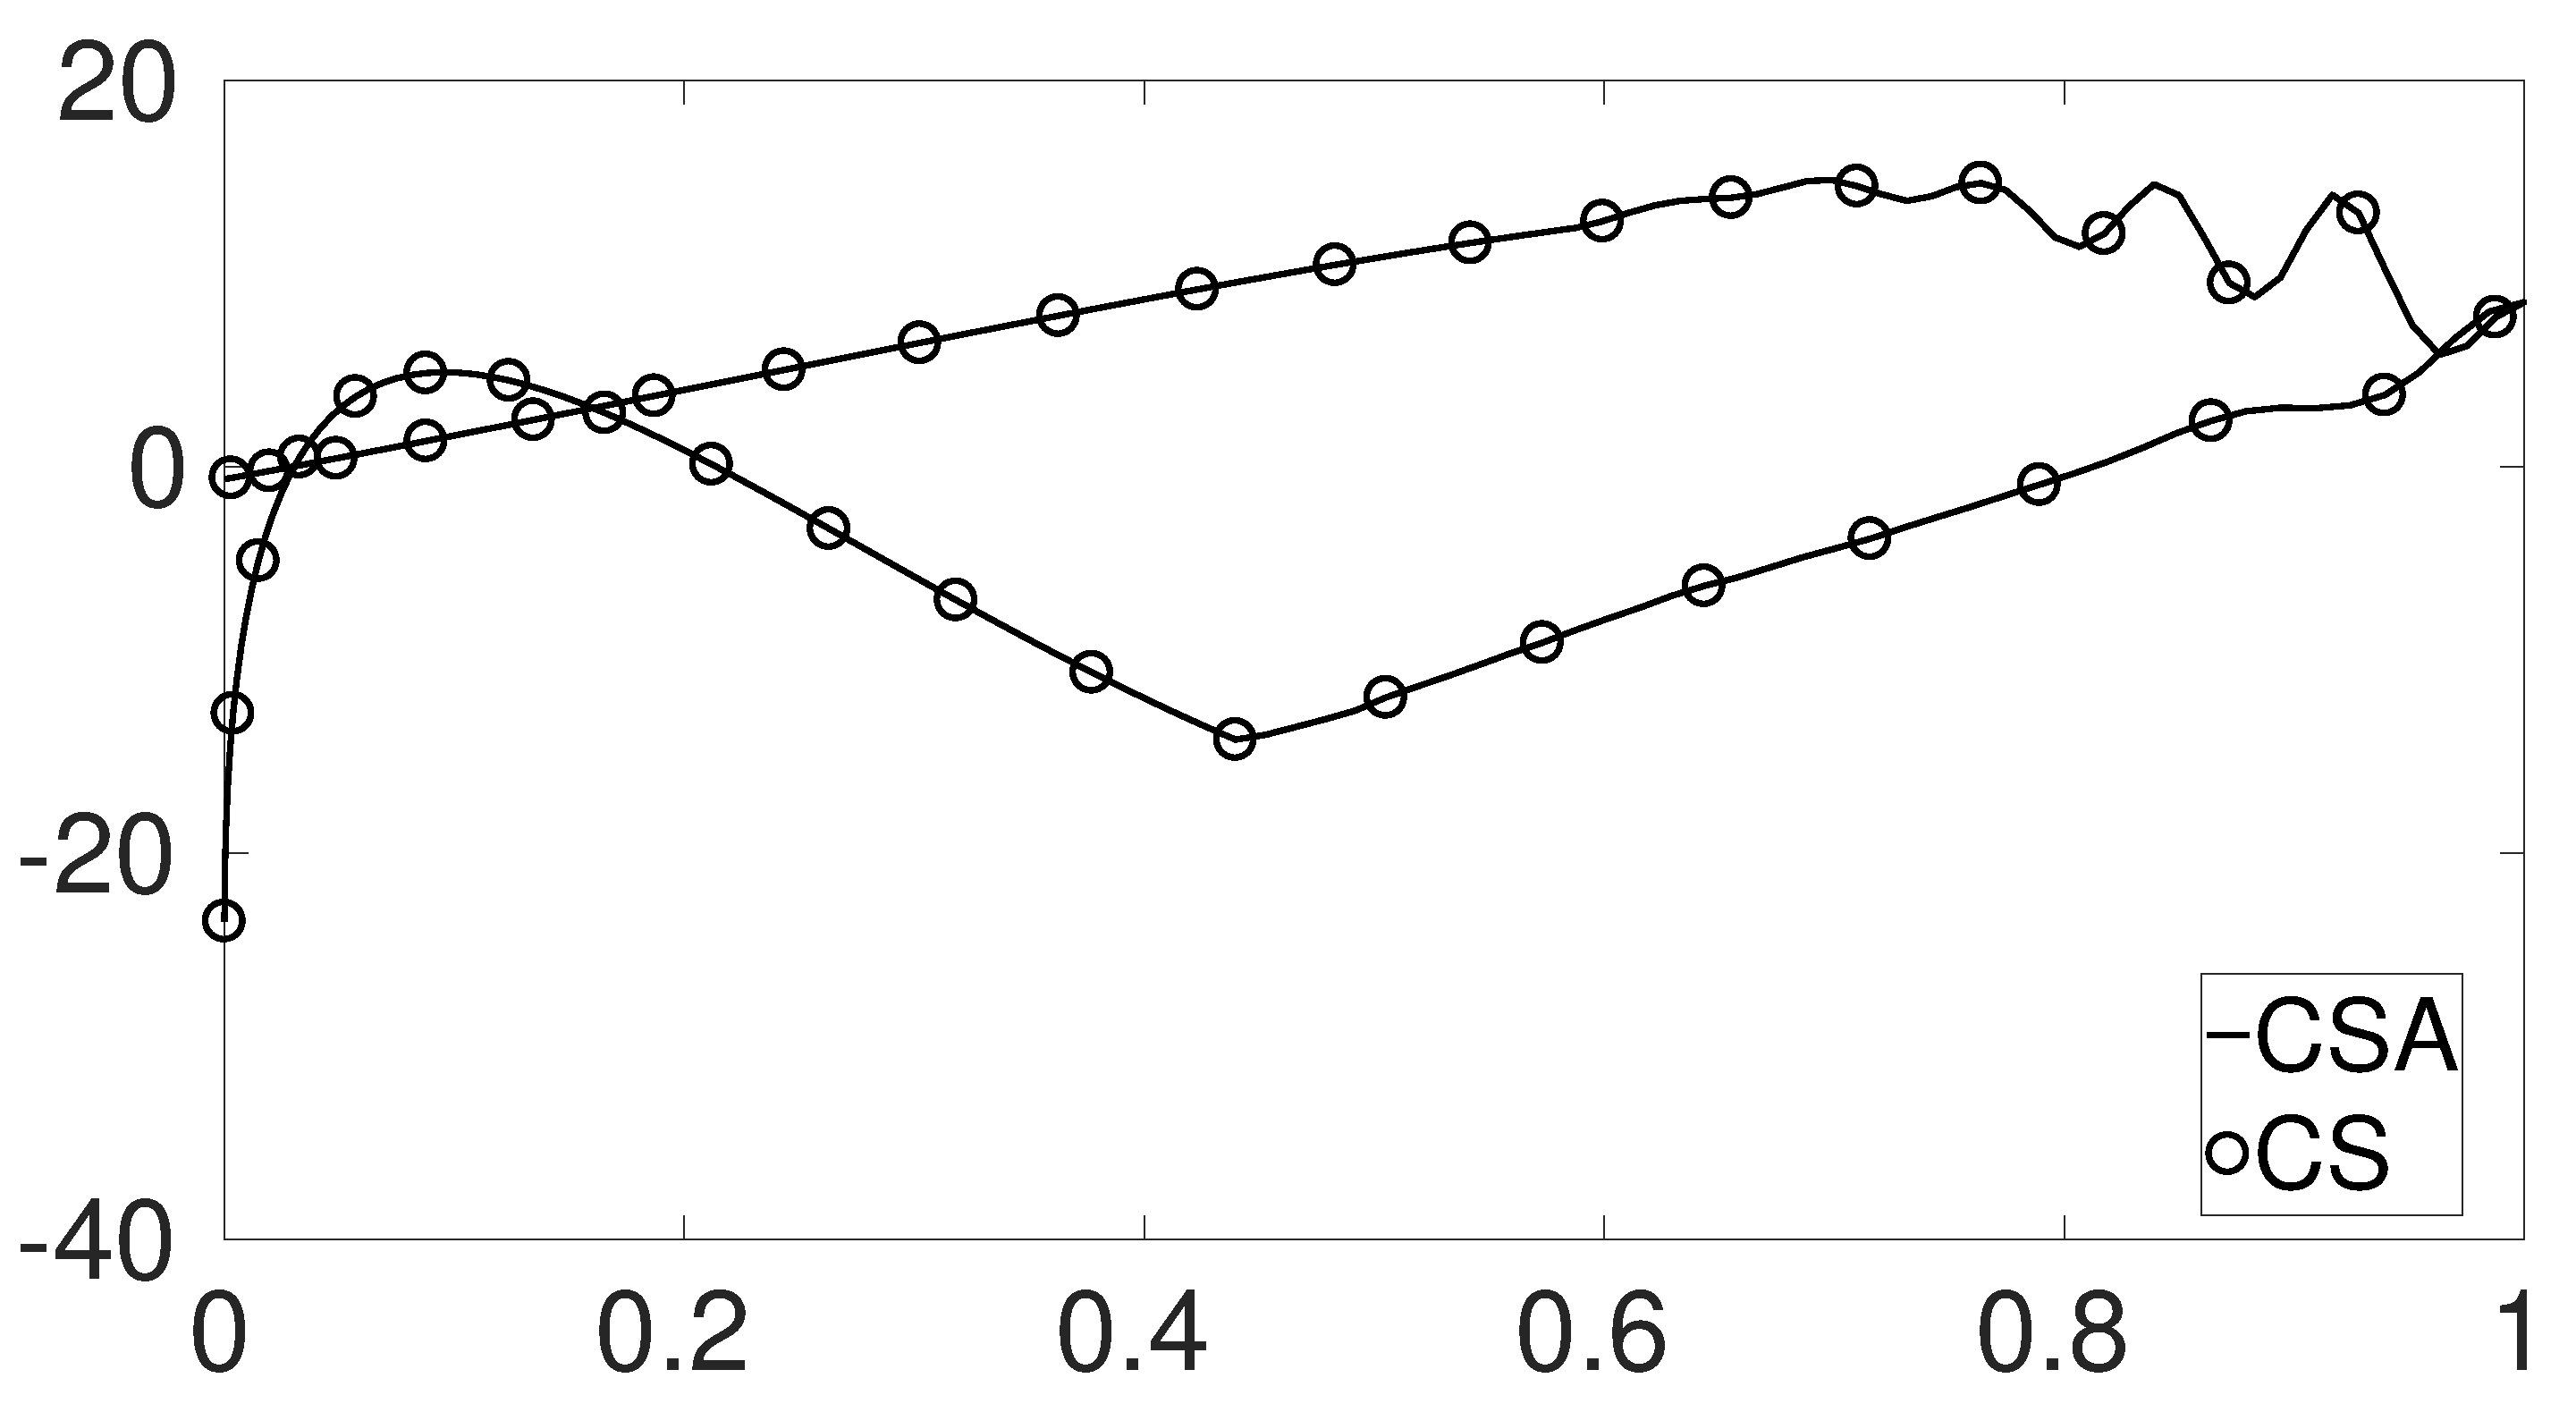
\includegraphics[height=4.0cm]{figure/RAE2822/sensitivity_RAE2822_bottomDV.eps}
	}
	\caption{RAE 2822 surface pressure shape sensitity results.}
	\label{fig:RAE2822sensitivity}
\end{figure}
%
The surface sensitivity result is used for the following formulation for a shape optimization of NACA 0012 airfoil. This benchmark test is based on the work done by Vassberg et al. \cite{vassberg2011systematic}.
%
\begin{align*}
	&\text{minimize: } C_d \\
	&\text{subject ot: } y \geq y_\text{baseline}  \quad \forall x \in [0, 1]
\end{align*}
%
The shape of the RAE 2822 airfoil will be optimized based on the pressure sensitivity results of Figure \ref{fig:RAE2822sensitivity} based on the following optimization problem.
%
\begin{align*}
	\text{minimize: } &C_d \\
	\text{subject ot: } &C_l = 0.824 \\
	&C_m \geq -0.092 \\
	&\text{Area} \geq \text{Area}_\text{initial}
\end{align*}
%
The sensitivity of lift, drag, and pitching coefficient with respect to shape design variable, $b$, are calculated by analytical differentiation. The sensitivity of lift coefficient is calculated as shown in Equation \eqref{eq:liftCoefficientSensitivity}.
%
\begin{equation}\label{eq:liftCoefficientSensitivity}
	C_L = \frac{2L}{\rho u^2 S} \Rightarrow \frac{d C_L}{db} = \frac{2 dL/db}{\rho u^2 S}
\end{equation}
%
Where $L$ is the lift force, $\rho$ is the fluid density, $u$ is the free stream velocity, and $S$ is a relevant area. The sensitivity of lift force with respect to shape design variable is calculated based on the information about surface pressure sensitivity as shown in Equation \eqref{eq:liftSensitivity}.
%
\begin{equation}\label{eq:liftSensitivity}
	L = \oint_\Gamma p d\Gamma \Rightarrow \frac{dL}{db} = \oint_\Gamma \frac{dp}{db} d\Gamma
\end{equation}
%
where $\Gamma$ is the entire surface of the airfoil, $p$ is the pressure on the airfoil surface, and $b$ is the shape design variable. The pressure sensitivity information of Figures \ref{fig:NACA0012sensitivity} and \ref{fig:RAE2822sensitivity} is used in Equation \eqref{eq:liftSensitivity} for the sensitivity calculation.
% ==========================================================================================
\section{Summary Remarks}
In this research, a continuum sensitivity analysis formulation is developed for the aerodynamic shape optimization. The flow is modeled with the Navier-Stokes equations. The solid boundaries are modeled using the continuum formulation of the IB method with an addition of a feedback forcing function in the Navier-Stokes equations to represent the effect of solid boundaries. Using this approach, we were able to decouple the fluid mesh description from the shape of the solid boundary. This method improves the robustness of the coupled high-fidelity simulations since no mesh deformation is needed to handle the solid region deformation. Moreover, the sensitivity analysis is simplified since the local and total sensitivities are equal for this formulation. A nonlinear mapping function is used to couple the fluid and solid domain (Eulerian and Lagrangian) grids and maps the data between these domains. As a requirement for continuum sensitivity analysis, the mapping function needs to be $\mathcal{C}^1$ continuous. This is satisfied by proposing a novel regularized delta function that has continuous derivatives. The applicability of the proposed function is demonstrated in this research.

The sensitivity analysis methodology is applied to two airfoil shape design problems. The results conform well with the complex step results. It should be noted that it's hard to capture the same effects using the body conformal approach for these problems. This is mainly due to the requirement for mesh deformation is said algorithms.
% ==========================================================================================
\section*{Acknowledgements}
The authors would like to acknowledge the support provided by the Air Force Research Laboratory through the contract FA8650-09-23938, the Collaborative Center for Multidisciplinary Sciences.
% References
\bibliographystyle{aiaa}
\bibliography{ref}


\end{document}